\documentclass[11pt]{article}

\usepackage[margin=1in]{geometry}
\usepackage{amsmath}
\usepackage{amssymb}
\usepackage{graphicx}
\usepackage{hyperref}
\usepackage{placeins}
\usepackage{subcaption}
\usepackage[T1]{fontenc}
\usepackage{lmodern}

\hypersetup{
  colorlinks=true,
  linkcolor=blue,
  urlcolor=blue,
  citecolor=blue
}

\renewcommand{\topfraction}{0.95}
\renewcommand{\bottomfraction}{0.95}
\renewcommand{\textfraction}{0.05}
\renewcommand{\floatpagefraction}{0.8}

\title{Perfect One-Step Rapid-Sine Scalar-Mixing Figures}
\author{}
\date{\today}

\begin{document}
\maketitle

\noindent
This note summarizes a matched set of frozen-velocity passive-scalar experiments in
two and three spatial dimensions. The two-dimensional runs use the stream-function
construction, the three-dimensional runs use the projection construction, and the
initial scalar field is a one-sided step: $\theta(x,0)=0$ on one side of the domain
and $\theta(x,0)=1$ on the other. Across both ensembles we scan the velocity
roughness exponent $\alpha$ and the scalar diffusivity $D$, then use the resulting
scalar power spectra and dissipation diagnostics to track how scalar regularity and
finite-time dissipation change across the parameter sweep.

\section{Setup and observables}
The scalar evolves under the advection-diffusion equation
\begin{equation}
  \partial_t \theta + u(x)\cdot \nabla \theta = D \Delta \theta,
\end{equation}
with a time-independent incompressible velocity field $u$. The velocity roughness is
parameterized by $\alpha$, with the shell-integrated velocity spectrum written as
\begin{equation}
  E_u(k) \propto k^{-(2\alpha+1)}.
\end{equation}
For each value of $\alpha$ we run a small diffusivity scan and analyze two outputs.
First, we infer a scalar regularity exponent $\beta$ from fitted theta-spectrum
slopes, using the same fitting convention as the plotting pipeline that produced the
figures below. Second, we track scalar dissipation through the finite-time integral
\begin{equation}
  \chi_D(T) = D \int_0^T \int |\nabla \theta(x,t)|^2 \, dx \, dt.
\end{equation}
The time-trace figures show when dissipation is active during the run, while the
integrated curves summarize the quantity relevant to the vanishing-diffusivity
question.

\begin{figure}[htbp]
  \centering
  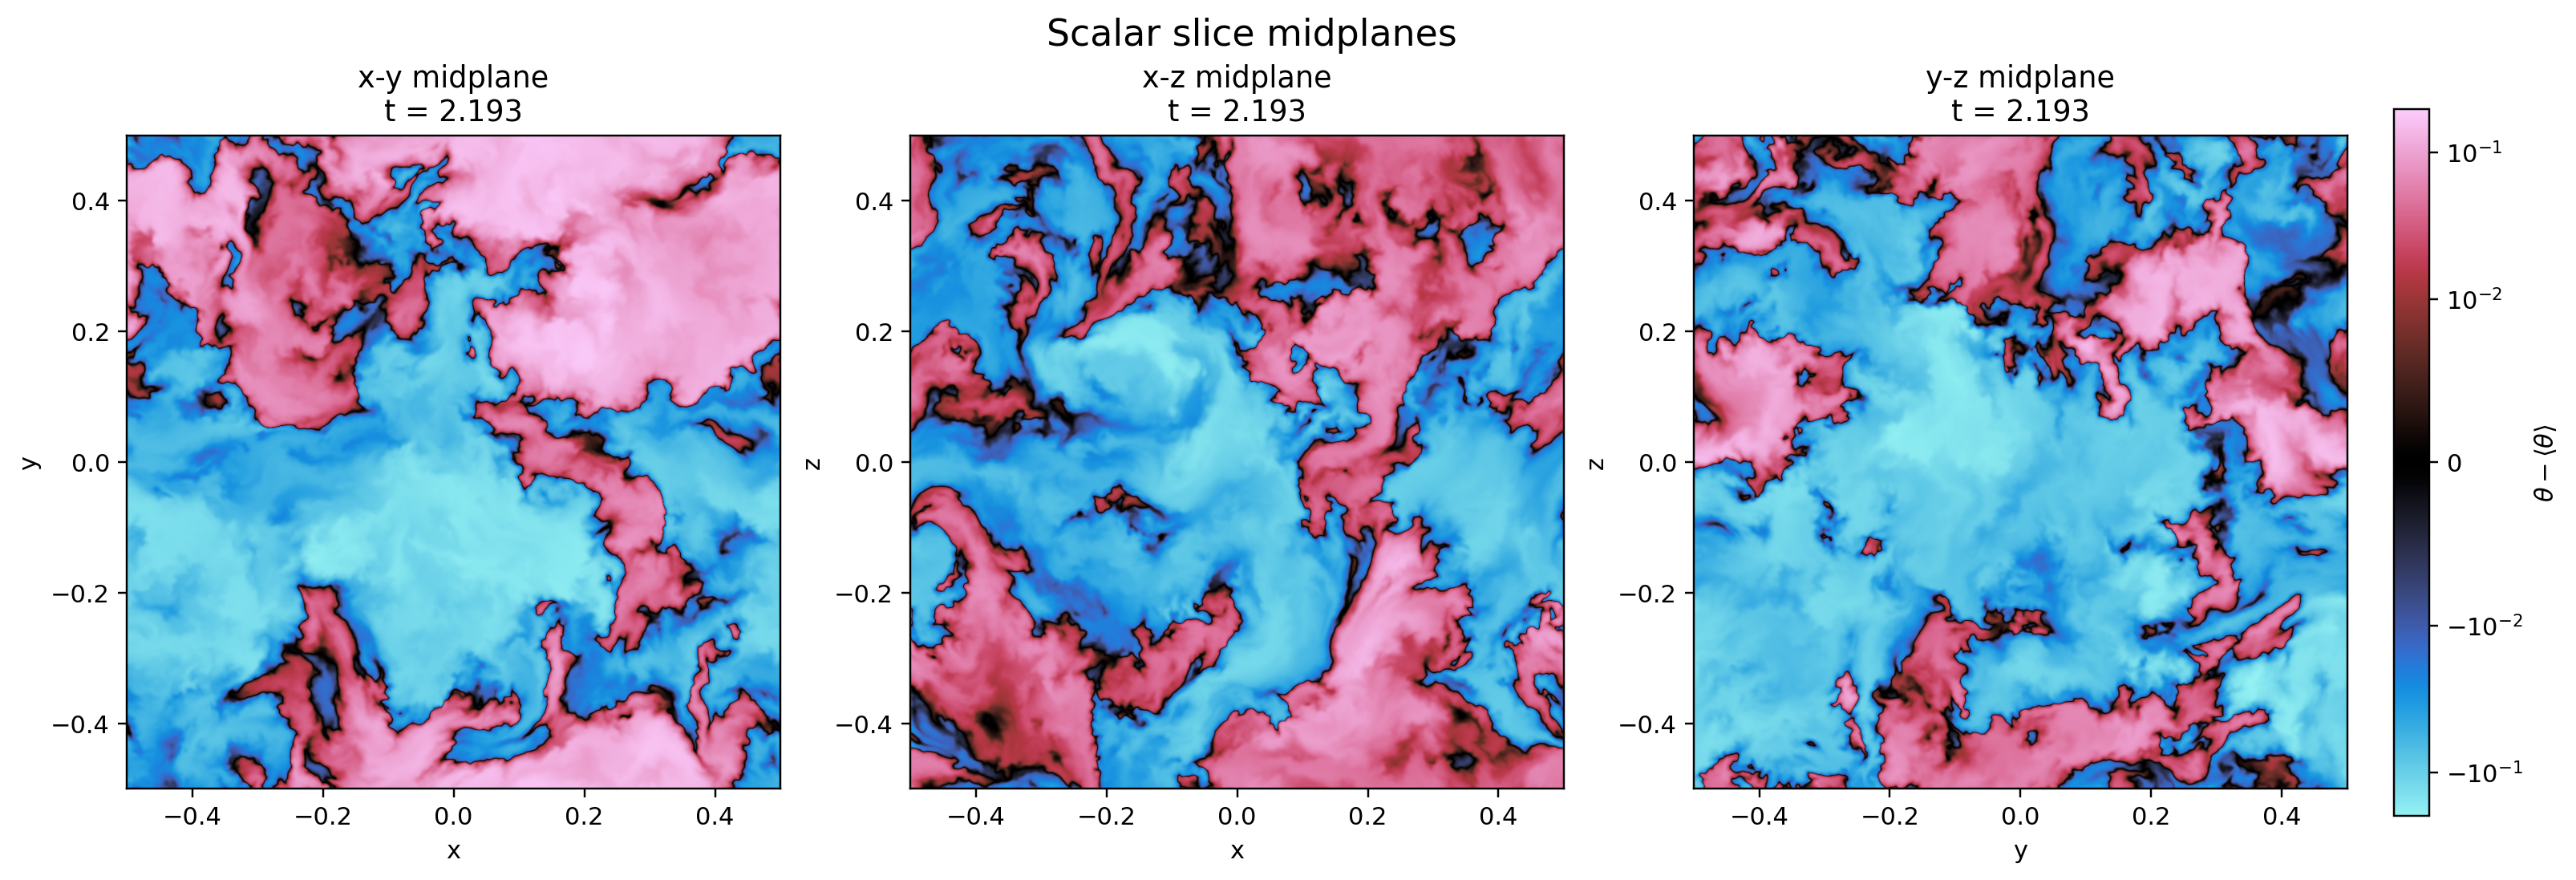
\includegraphics[width=\textwidth]{figures_perfect1_step_rapidsine/scalar_slice_midplanes_smix3d_1024_mb256_projection_perfect_expo4o3_sd3p16e-4_seed51825_2scalars_s_00.png}

  \vspace{0.75em}

  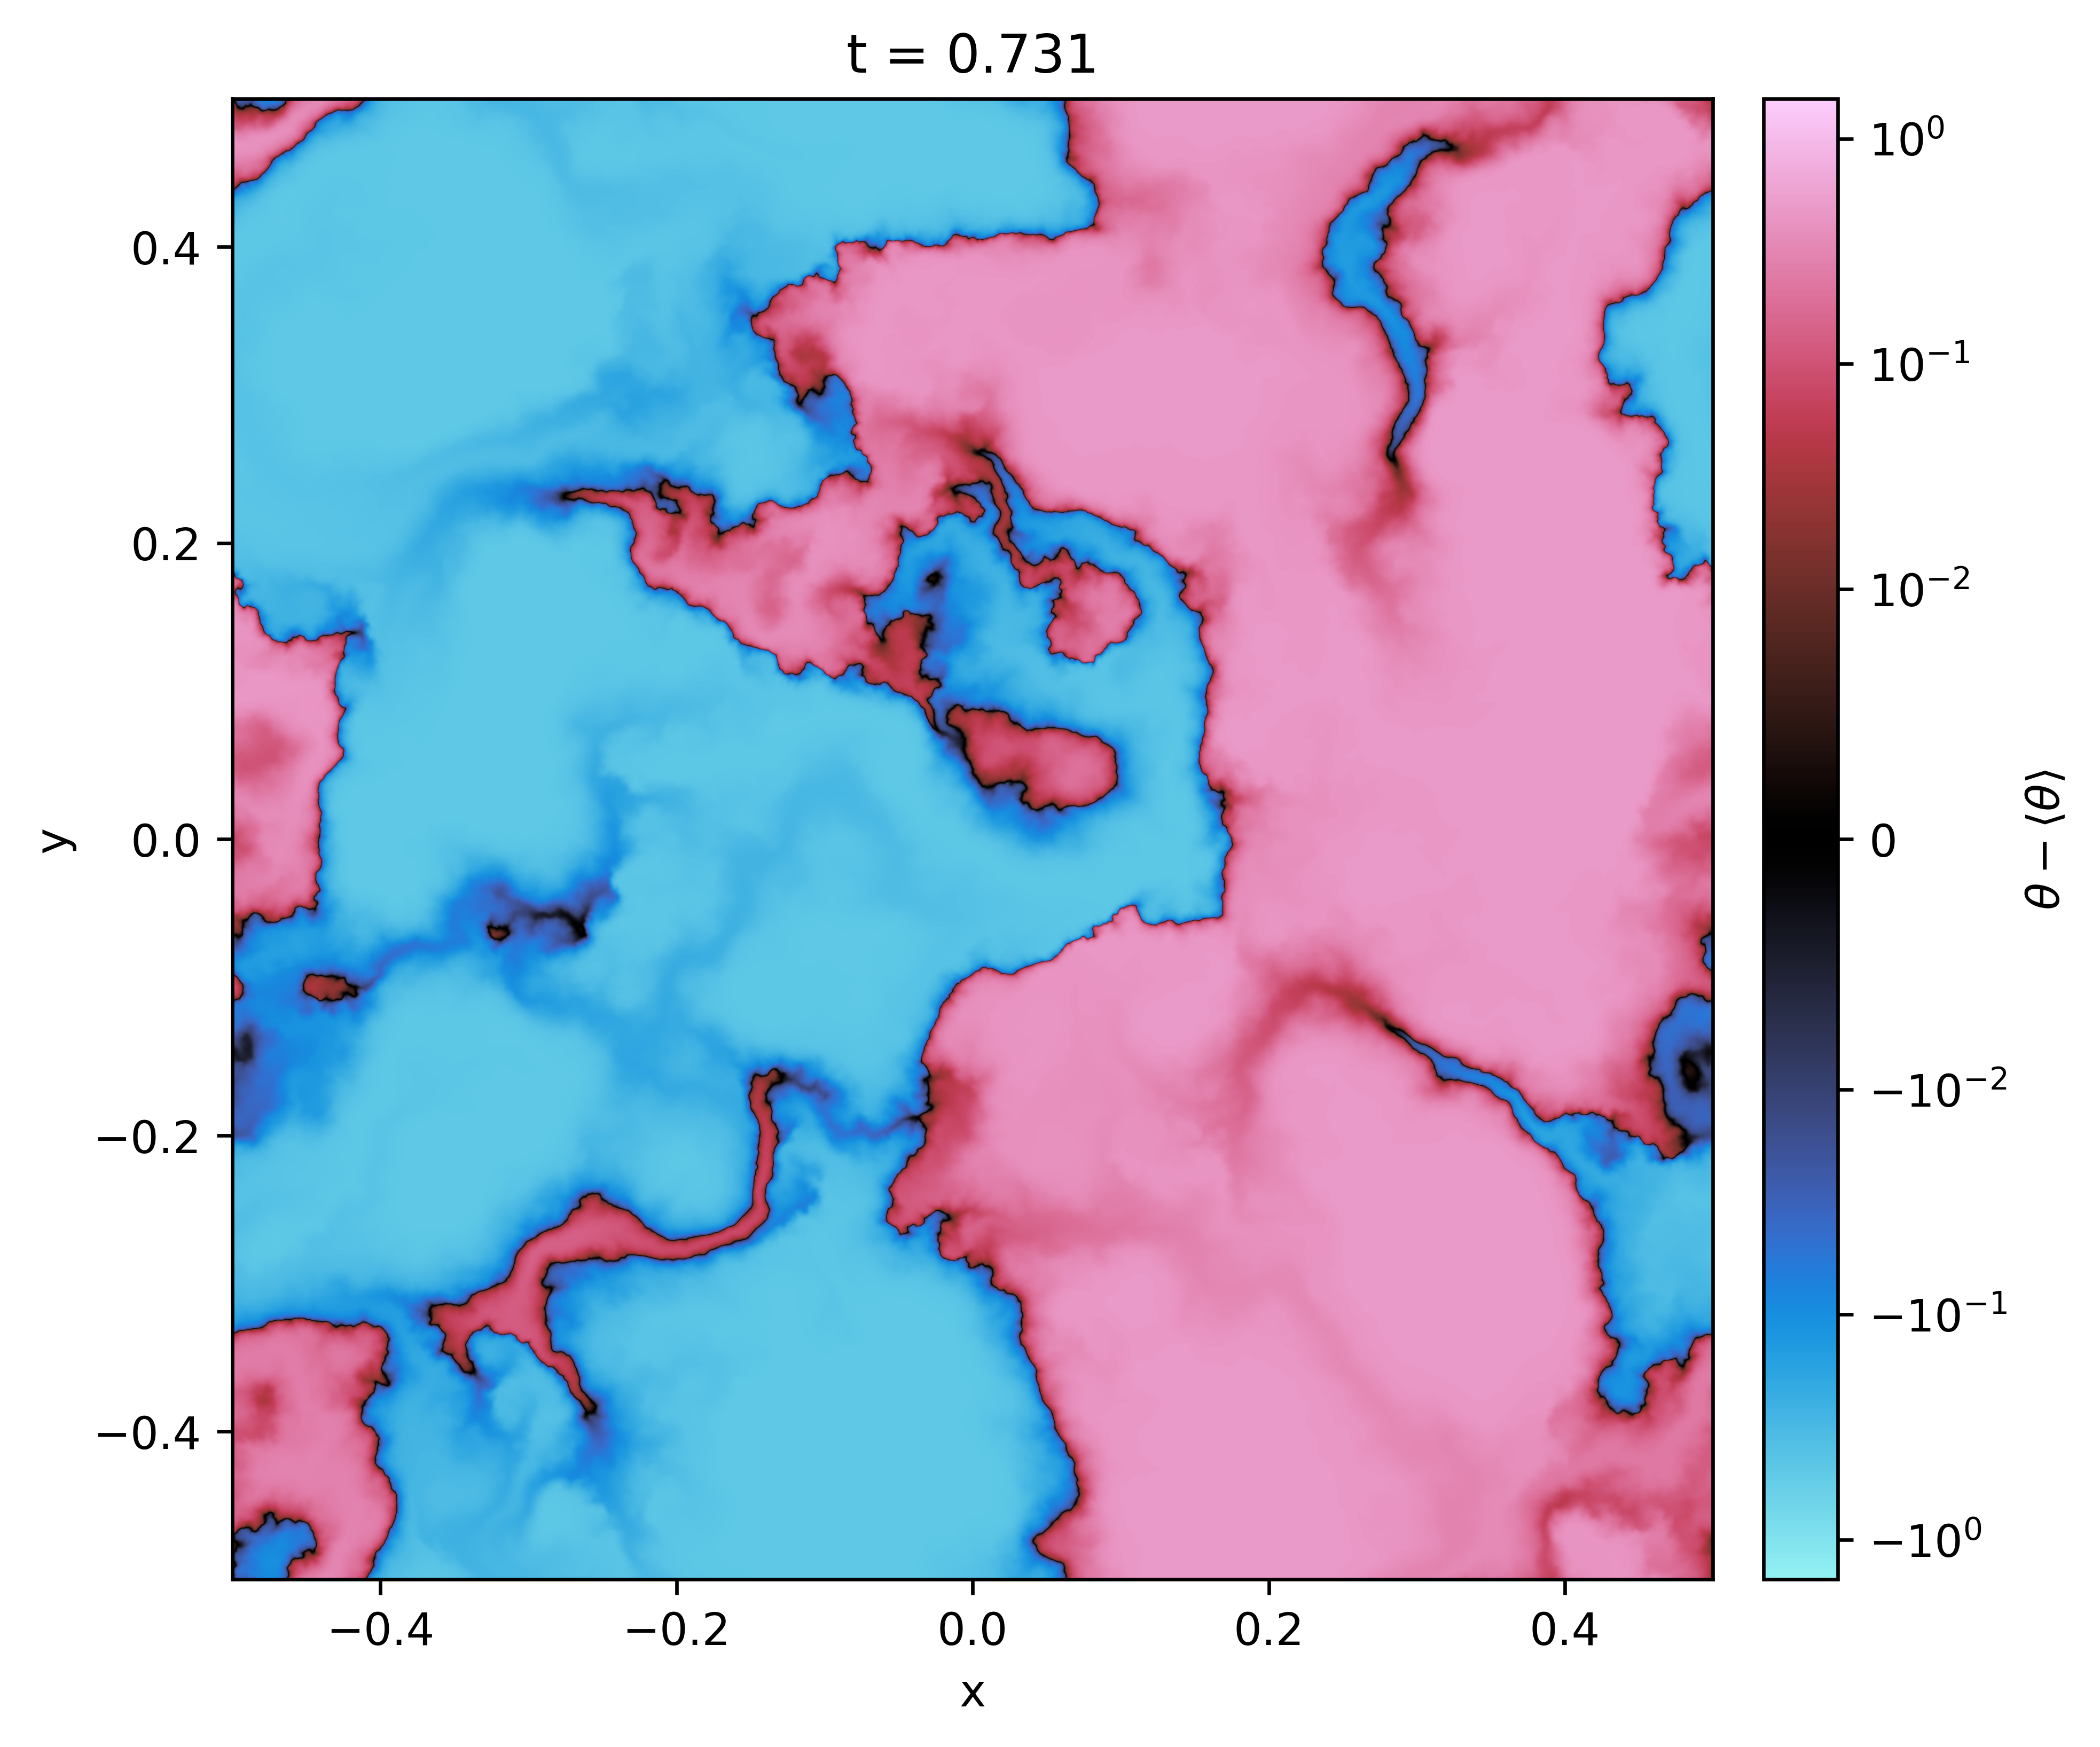
\includegraphics[width=0.62\textwidth]{figures_perfect1_step_rapidsine/smix2d_4096_mb1024_stream_perfect_expo4o3_sd3p16e-4_seed51825_2scalars_frame_0003.png}
  \caption{Representative scalar maps from the two ensembles. The upper panel shows
  the three orthogonal midplane slices from a 3D projection run, while the lower
  panel shows a 2D stream-function run. These images are included only as qualitative
  morphology examples of the folded step profile after advection and diffusion; they
  are not meant to summarize the full $\alpha$-$D$ scan by themselves.}
  \label{fig:maps}
\end{figure}

\section{Diffusivity window}
The original scan covered very small diffusivities, but not all of those values are
equally informative. If the velocity increments scale like
\begin{equation}
  \delta v(l) \sim U_{\mathrm{rms}} \left( \frac{l}{L} \right)^{\alpha},
\end{equation}
then the diffusive and advective times at scale $l$ are
\begin{equation}
  t_{\mathrm{diff}}(l) = \frac{l^2}{D},
  \qquad
  t_{\mathrm{adv}}(l) = \frac{l}{\delta v(l)}
  = \frac{L}{U_{\mathrm{rms}}} \left( \frac{l}{L} \right)^{1-\alpha}.
\end{equation}
The diffusive cutoff scale $\eta_D$ is defined by
$t_{\mathrm{diff}}(\eta_D)=t_{\mathrm{adv}}(\eta_D)$, which gives
\begin{equation}
  \frac{\eta_D}{L}
  = \left( \frac{D}{L U_{\mathrm{rms}}} \right)^{\frac{1}{1+\alpha}}.
\end{equation}
On a finite grid the useful regime is the one in which the diffusive cutoff lies
between the box scale and the smallest resolved scale,
$l_{\min} \ll \eta_D \ll L$. The upper edge is therefore
$D_{\max} \sim L U_{\mathrm{rms}}$, while the lower edge comes from setting
$\eta_D = l_{\min}$:
\begin{equation}
  D_{\min} = L U_{\mathrm{rms}} \left( \frac{l_{\min}}{L} \right)^{1+\alpha}.
\end{equation}
For the present runs one can think of $L=1/2$ and $l_{\min}=1/k_{\max}$, so the
allowed lower edge moves rapidly with both $\alpha$ and the effective resolution. As
a concrete guide, if $l_{\min}/L \sim 10^{-3}$ then
$D_{\min}\sim 10^{-3}$ for $\alpha=0$,
$D_{\min}\sim 10^{-4}$ for $\alpha=1/3$, and
$D_{\min}\sim 10^{-6}$ for $\alpha=1$.
The new summary figure below adds a tenfold safety buffer on both sides, so the
preferred range is roughly
\begin{equation}
  10 D_{\min} \lesssim D \lesssim \frac{D_{\max}}{10}.
\end{equation}
This provides the main caution for the rest of the note: a substantial fraction of
the earlier runs probed diffusivities below the preferred window, especially for the
rougher velocity fields and the larger effective values of $k_{\max}$.

\begin{figure}[htbp]
  \centering
  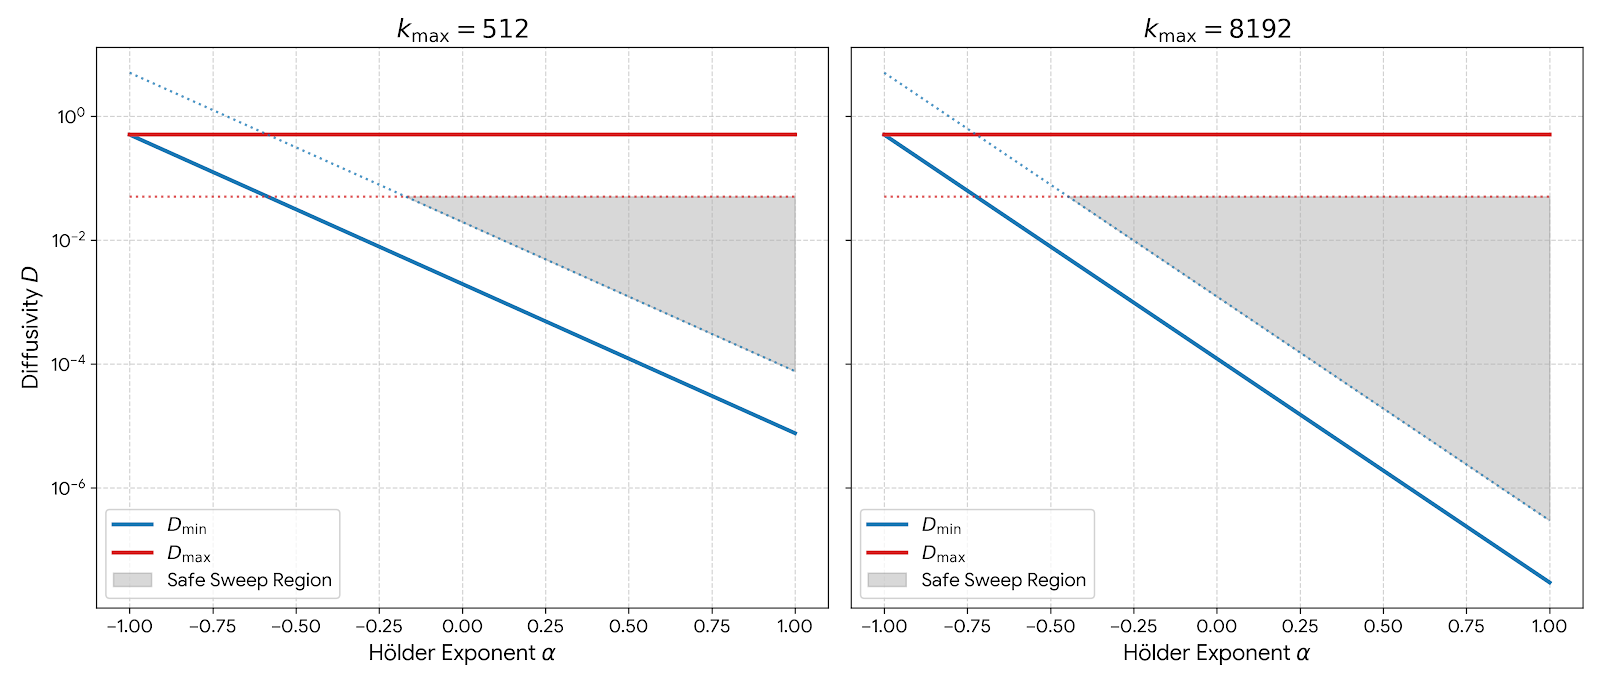
\includegraphics[width=\textwidth]{figures_perfect1_step_rapidsine/diffusivity_range.png}
  \caption{Admissible diffusivity range as a function of the velocity roughness
  exponent $\alpha$. The left panel uses $k_{\max}=512$ and the right panel uses
  $k_{\max}=8192$. In both panels the solid blue curve marks $D_{\min}$, the solid
  red line marks $D_{\max}$, the dotted curves show the tenfold buffer away from
  those limits, and the shaded region marks the intended safe sweep window. This
  figure is the reference for interpreting the later dissipation plots: many of the
  originally sampled diffusivities fall below the buffered lower limit.}
  \label{fig:diff-range}
\end{figure}

\section{Spectral regularity}
The first set of quantitative diagnostics comes from the theta power spectra. Figure
\ref{fig:theta-spectra} shows representative shared-time spectra for a single
diffusivity, $D=3.16\times10^{-4}$, across the roughness scan. The fitted slopes in
these spectra are then converted, using the existing plotting convention, into the
scalar regularity exponent $\beta$ summarized in Figure \ref{fig:beta-alpha}. The
goal here is descriptive rather than doctrinal: the figures show how the inferred
scalar roughness varies with the imposed velocity roughness, but they do not by
themselves settle whether any one asymptotic prediction should be treated as exact.

\begin{figure}[htbp]
  \centering
  \begin{subfigure}[t]{0.49\textwidth}
    \centering
    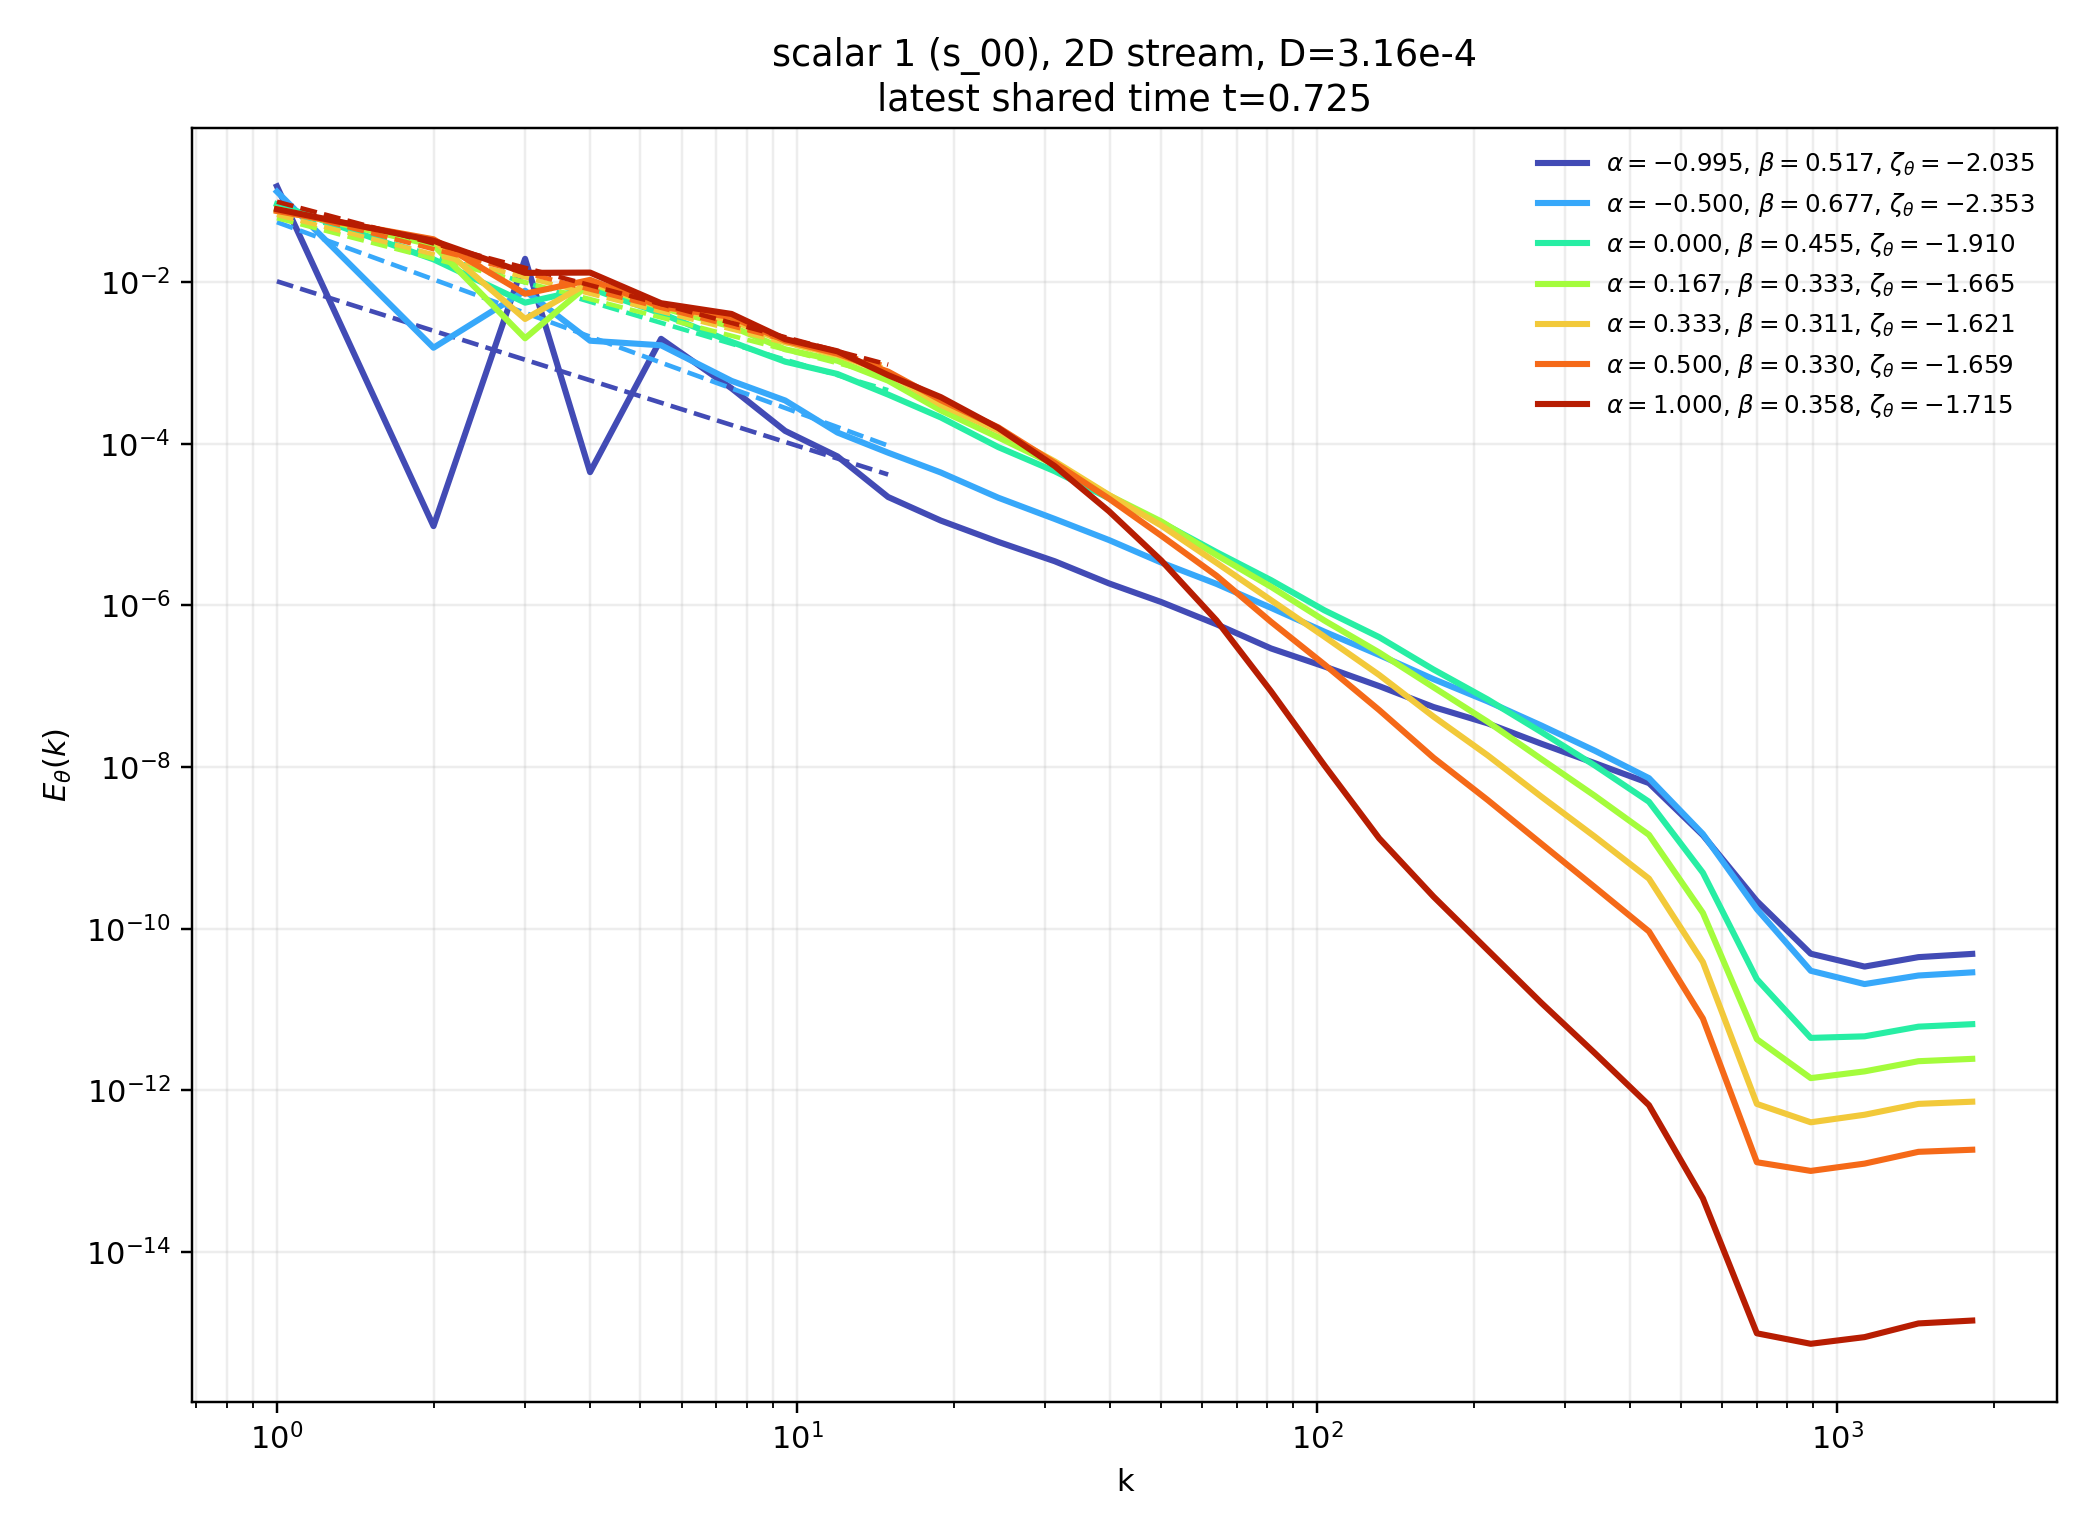
\includegraphics[width=\textwidth]{figures_perfect1_step_rapidsine/shared_time_theta_spectra_s_00_2d_stream_sd3p16em4_compare_alpha_with_fits.png}
    \caption{2D stream-function runs.}
  \end{subfigure}
  \hfill
  \begin{subfigure}[t]{0.49\textwidth}
    \centering
    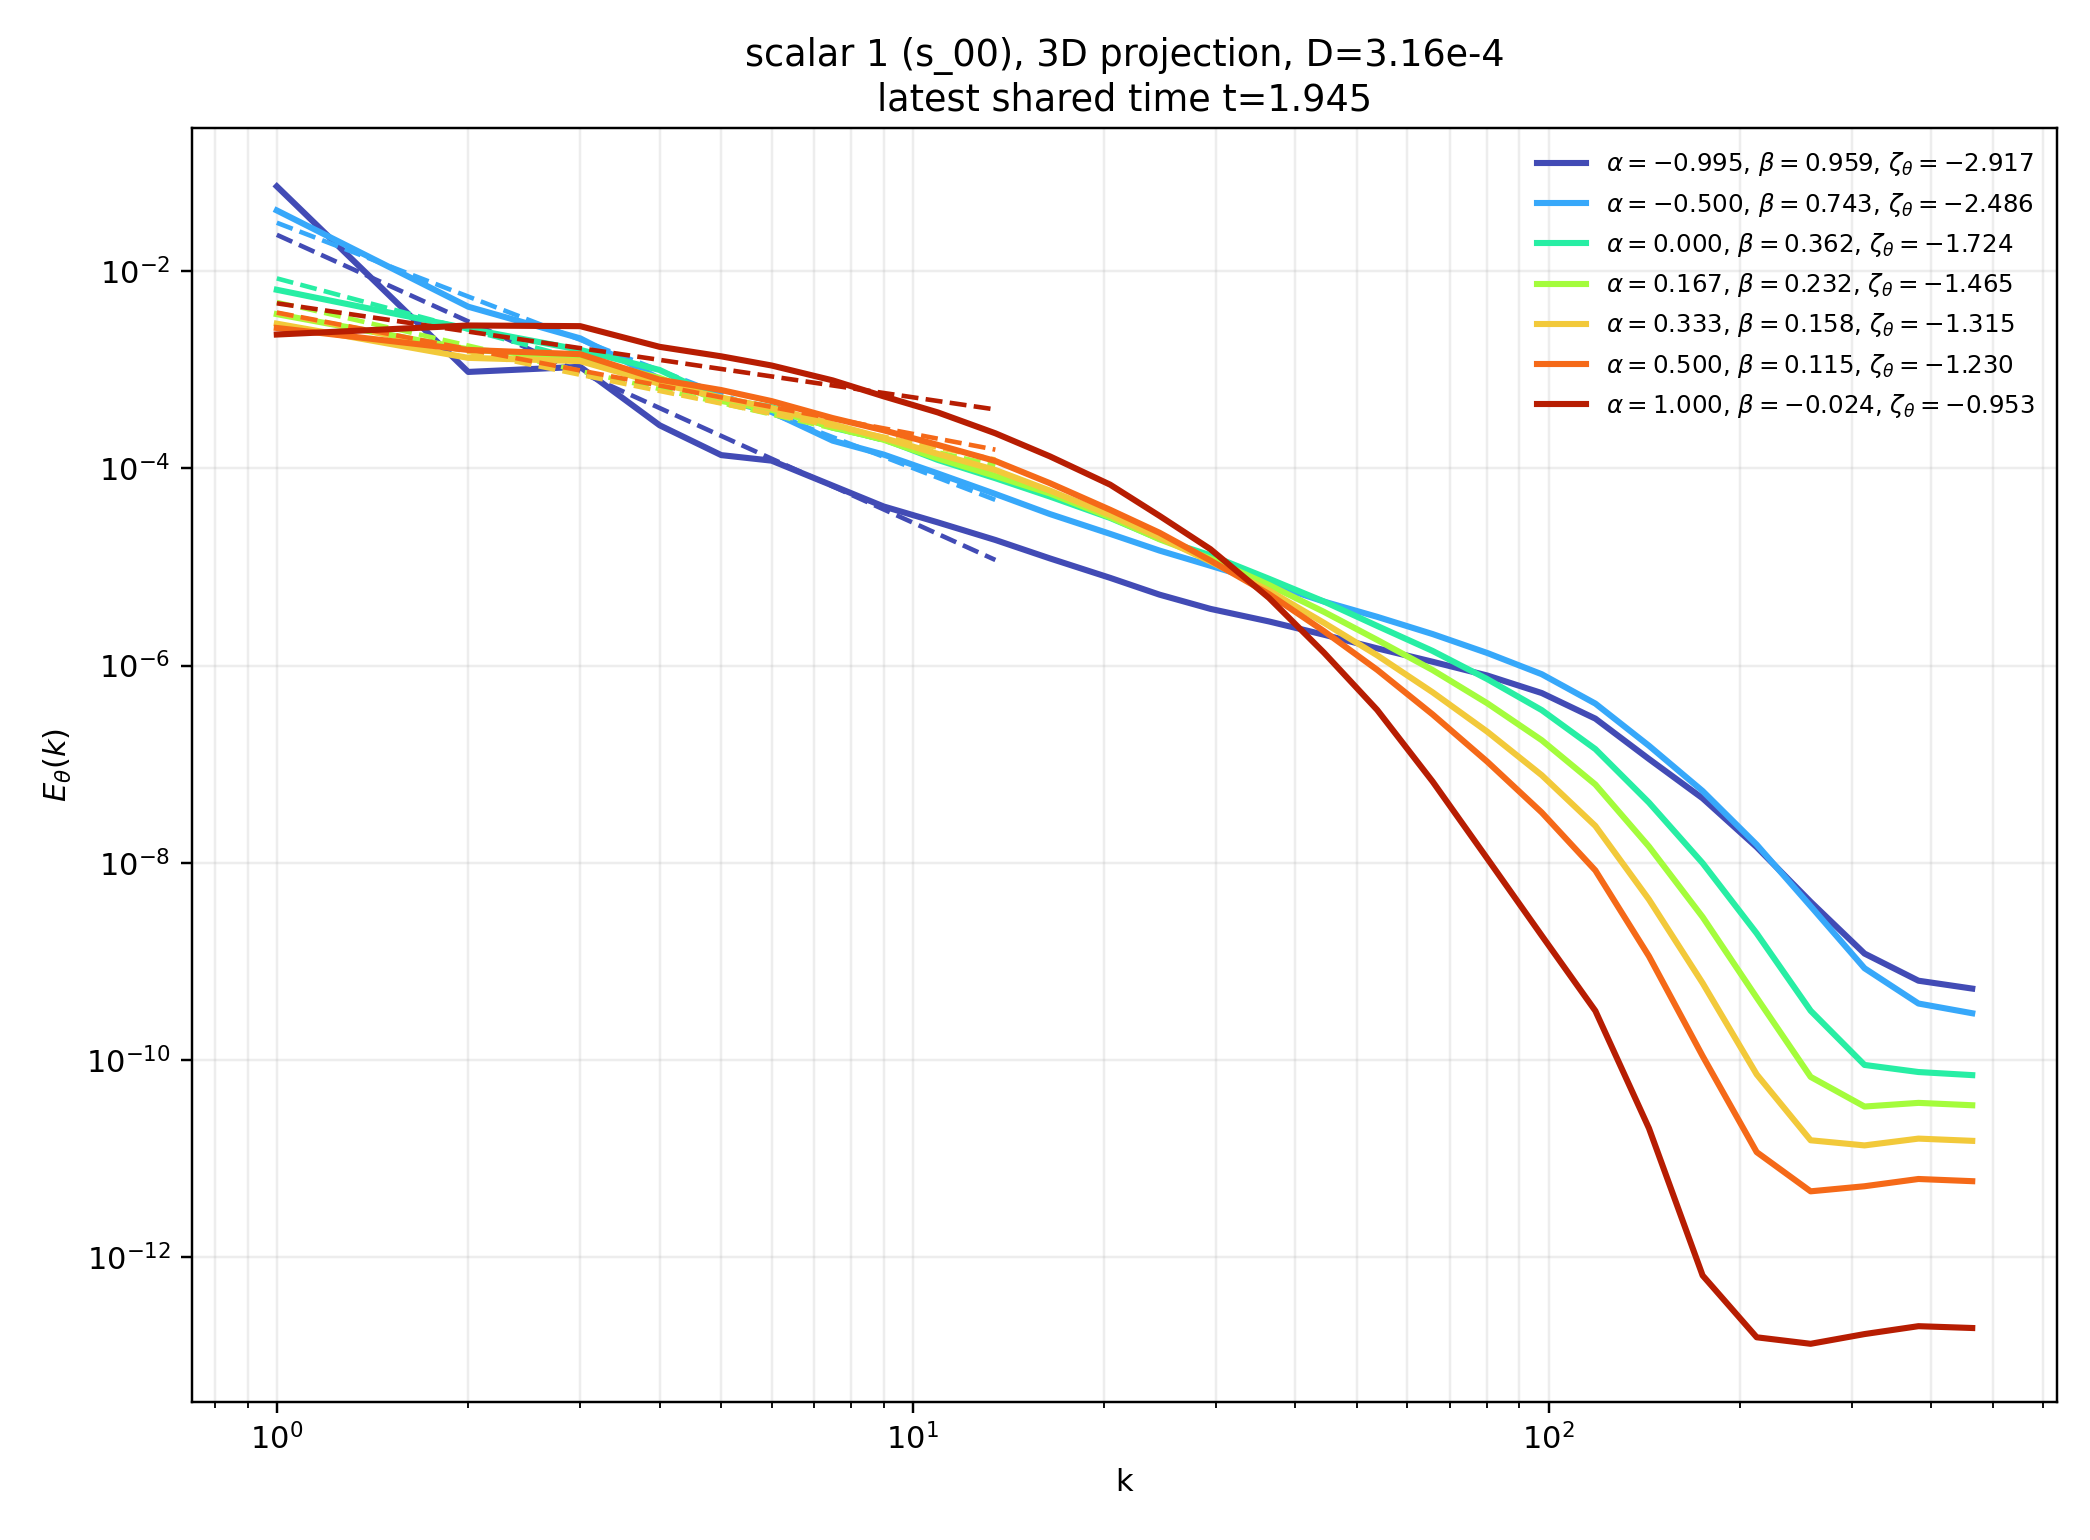
\includegraphics[width=\textwidth]{figures_perfect1_step_rapidsine/shared_time_theta_spectra_s_00_3d_projection_sd3p16em4_compare_alpha_with_fits.png}
    \caption{3D projection runs.}
  \end{subfigure}
  \caption{Representative theta power spectra at shared time for
  $D=3.16\times10^{-4}$. These plots show the fitted scalar power-law slopes used to
  infer the scalar regularity trend across the roughness scan.}
  \label{fig:theta-spectra}
\end{figure}

\begin{figure}[htbp]
  \centering
  \begin{subfigure}[t]{0.49\textwidth}
    \centering
    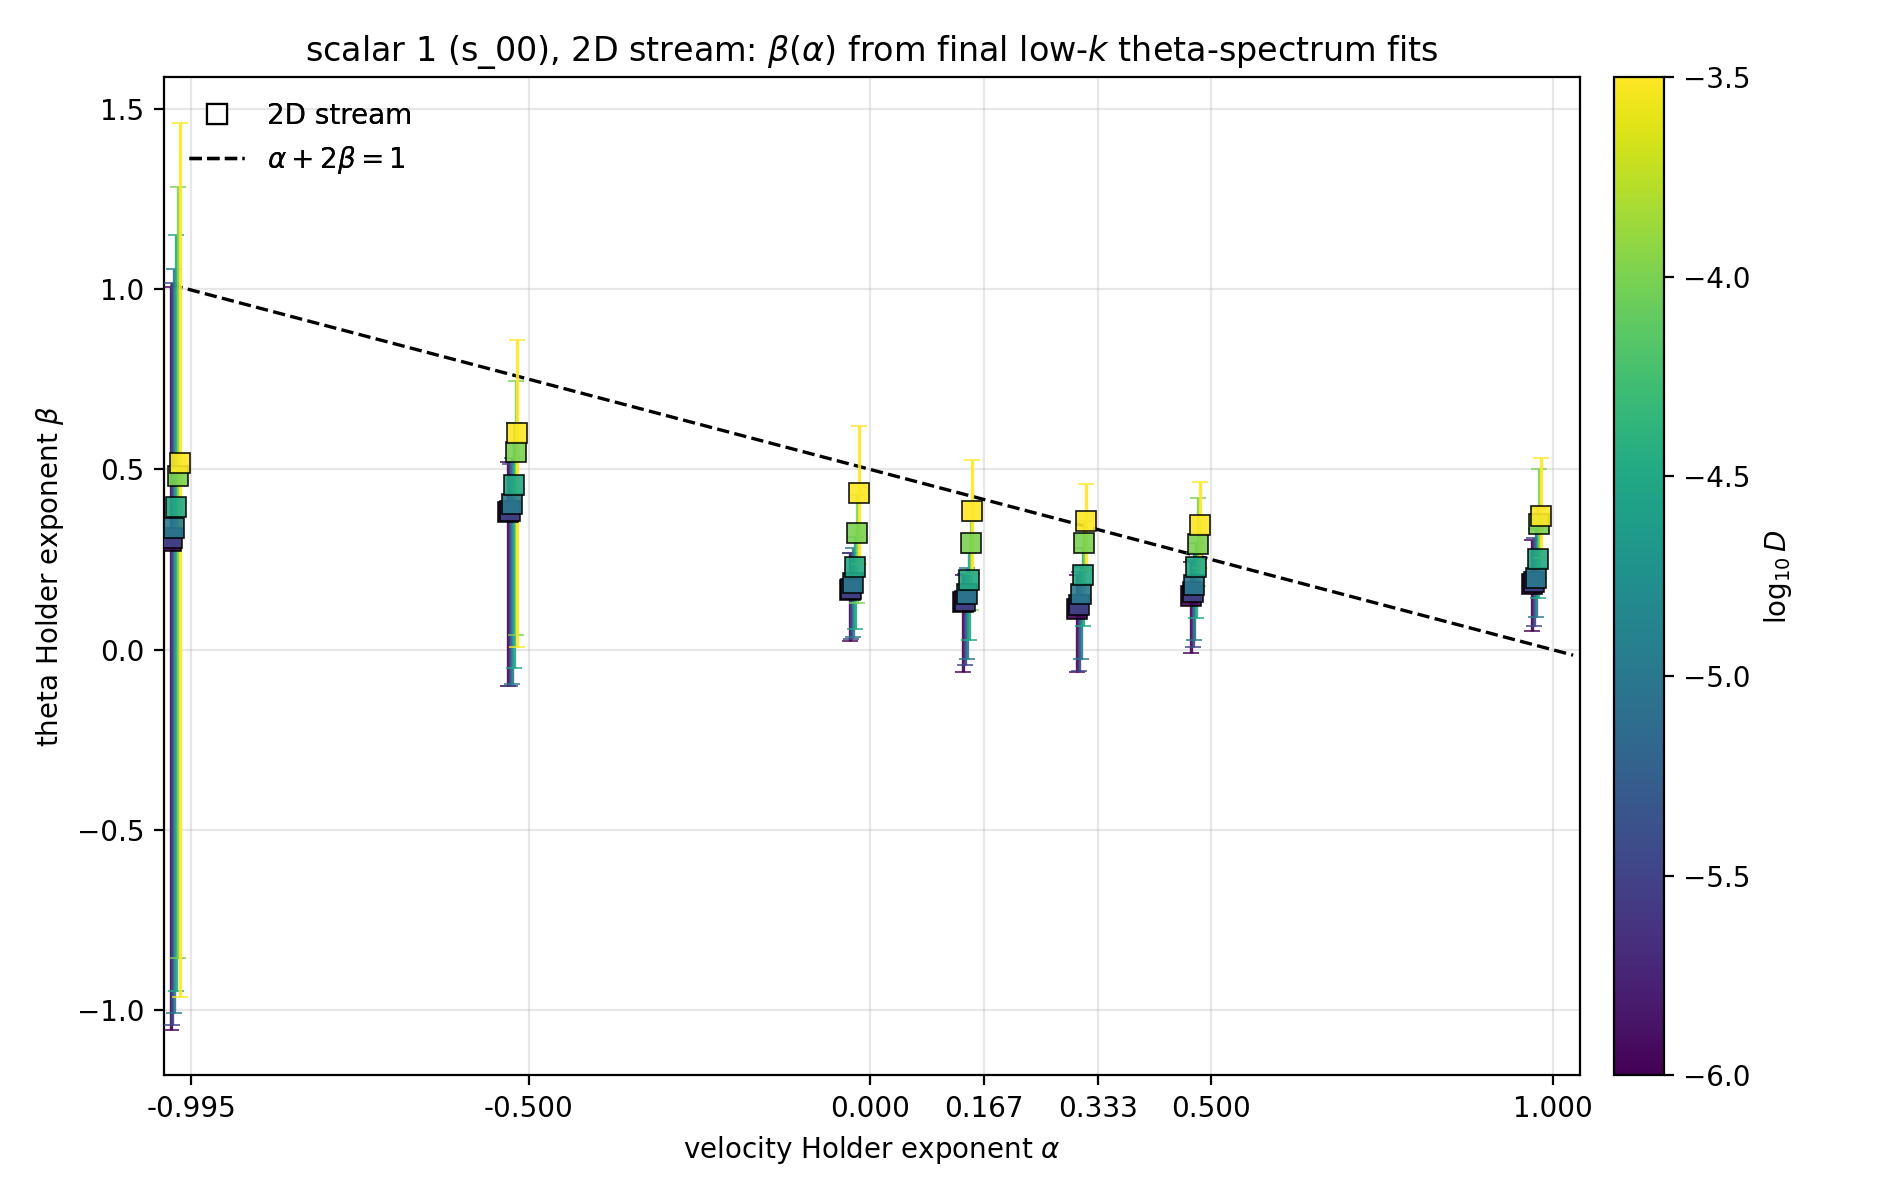
\includegraphics[width=\textwidth]{figures_perfect1_step_rapidsine/beta_vs_alpha_s_00_2d_stream.png}
    \caption{2D stream-function runs.}
  \end{subfigure}
  \hfill
  \begin{subfigure}[t]{0.49\textwidth}
    \centering
    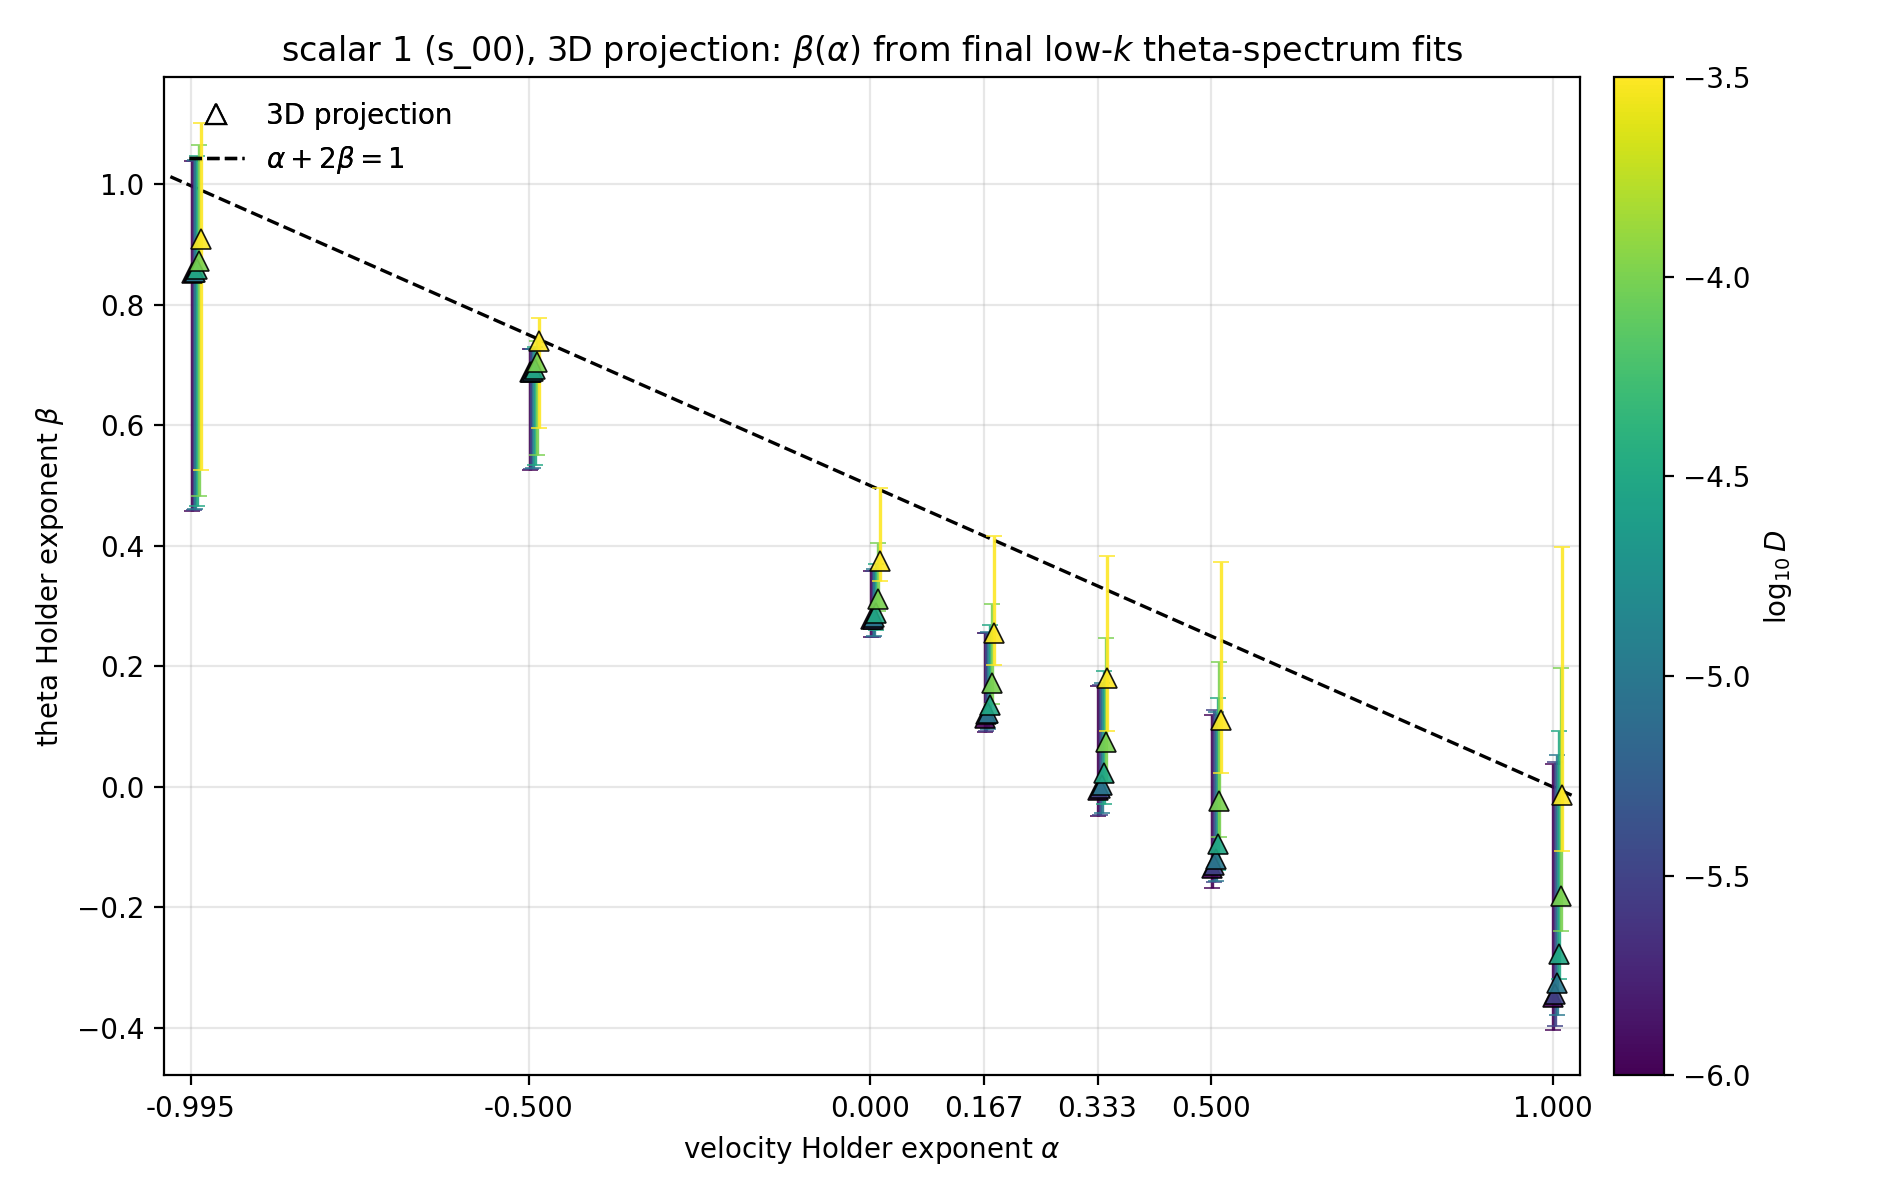
\includegraphics[width=\textwidth]{figures_perfect1_step_rapidsine/beta_vs_alpha_s_00_3d_projection.png}
    \caption{3D projection runs.}
  \end{subfigure}
  \caption{Inferred scalar regularity exponent $\beta$ as a function of the velocity
  roughness exponent $\alpha$. These summary plots condense the spectral fits across
  the scan and provide the cleanest view of how scalar roughness responds to the
  imposed velocity roughness in the two ensembles.}
  \label{fig:beta-alpha}
\end{figure}

\section{Dissipation diagnostics}
The dissipation plots separate two related questions. The instantaneous curves in
Figure \ref{fig:chi-time} show when dissipation is active during the finite
observation window and how that activity shifts across the roughness scan. The
integrated curves in Figure \ref{fig:chi-int} are the finite-time quantity directly
relevant to anomalous dissipation. Those integrated curves must be read together with
the admissible-diffusivity window in Figure \ref{fig:diff-range}: the black vertical
lines in the integrated plots mark the estimated $D_{\min}$ threshold, and values to
the left of those lines lie outside the preferred regime indicated by the buffered
range figure.

\begin{figure}[p]
  \centering
  \begin{subfigure}[t]{\textwidth}
    \centering
    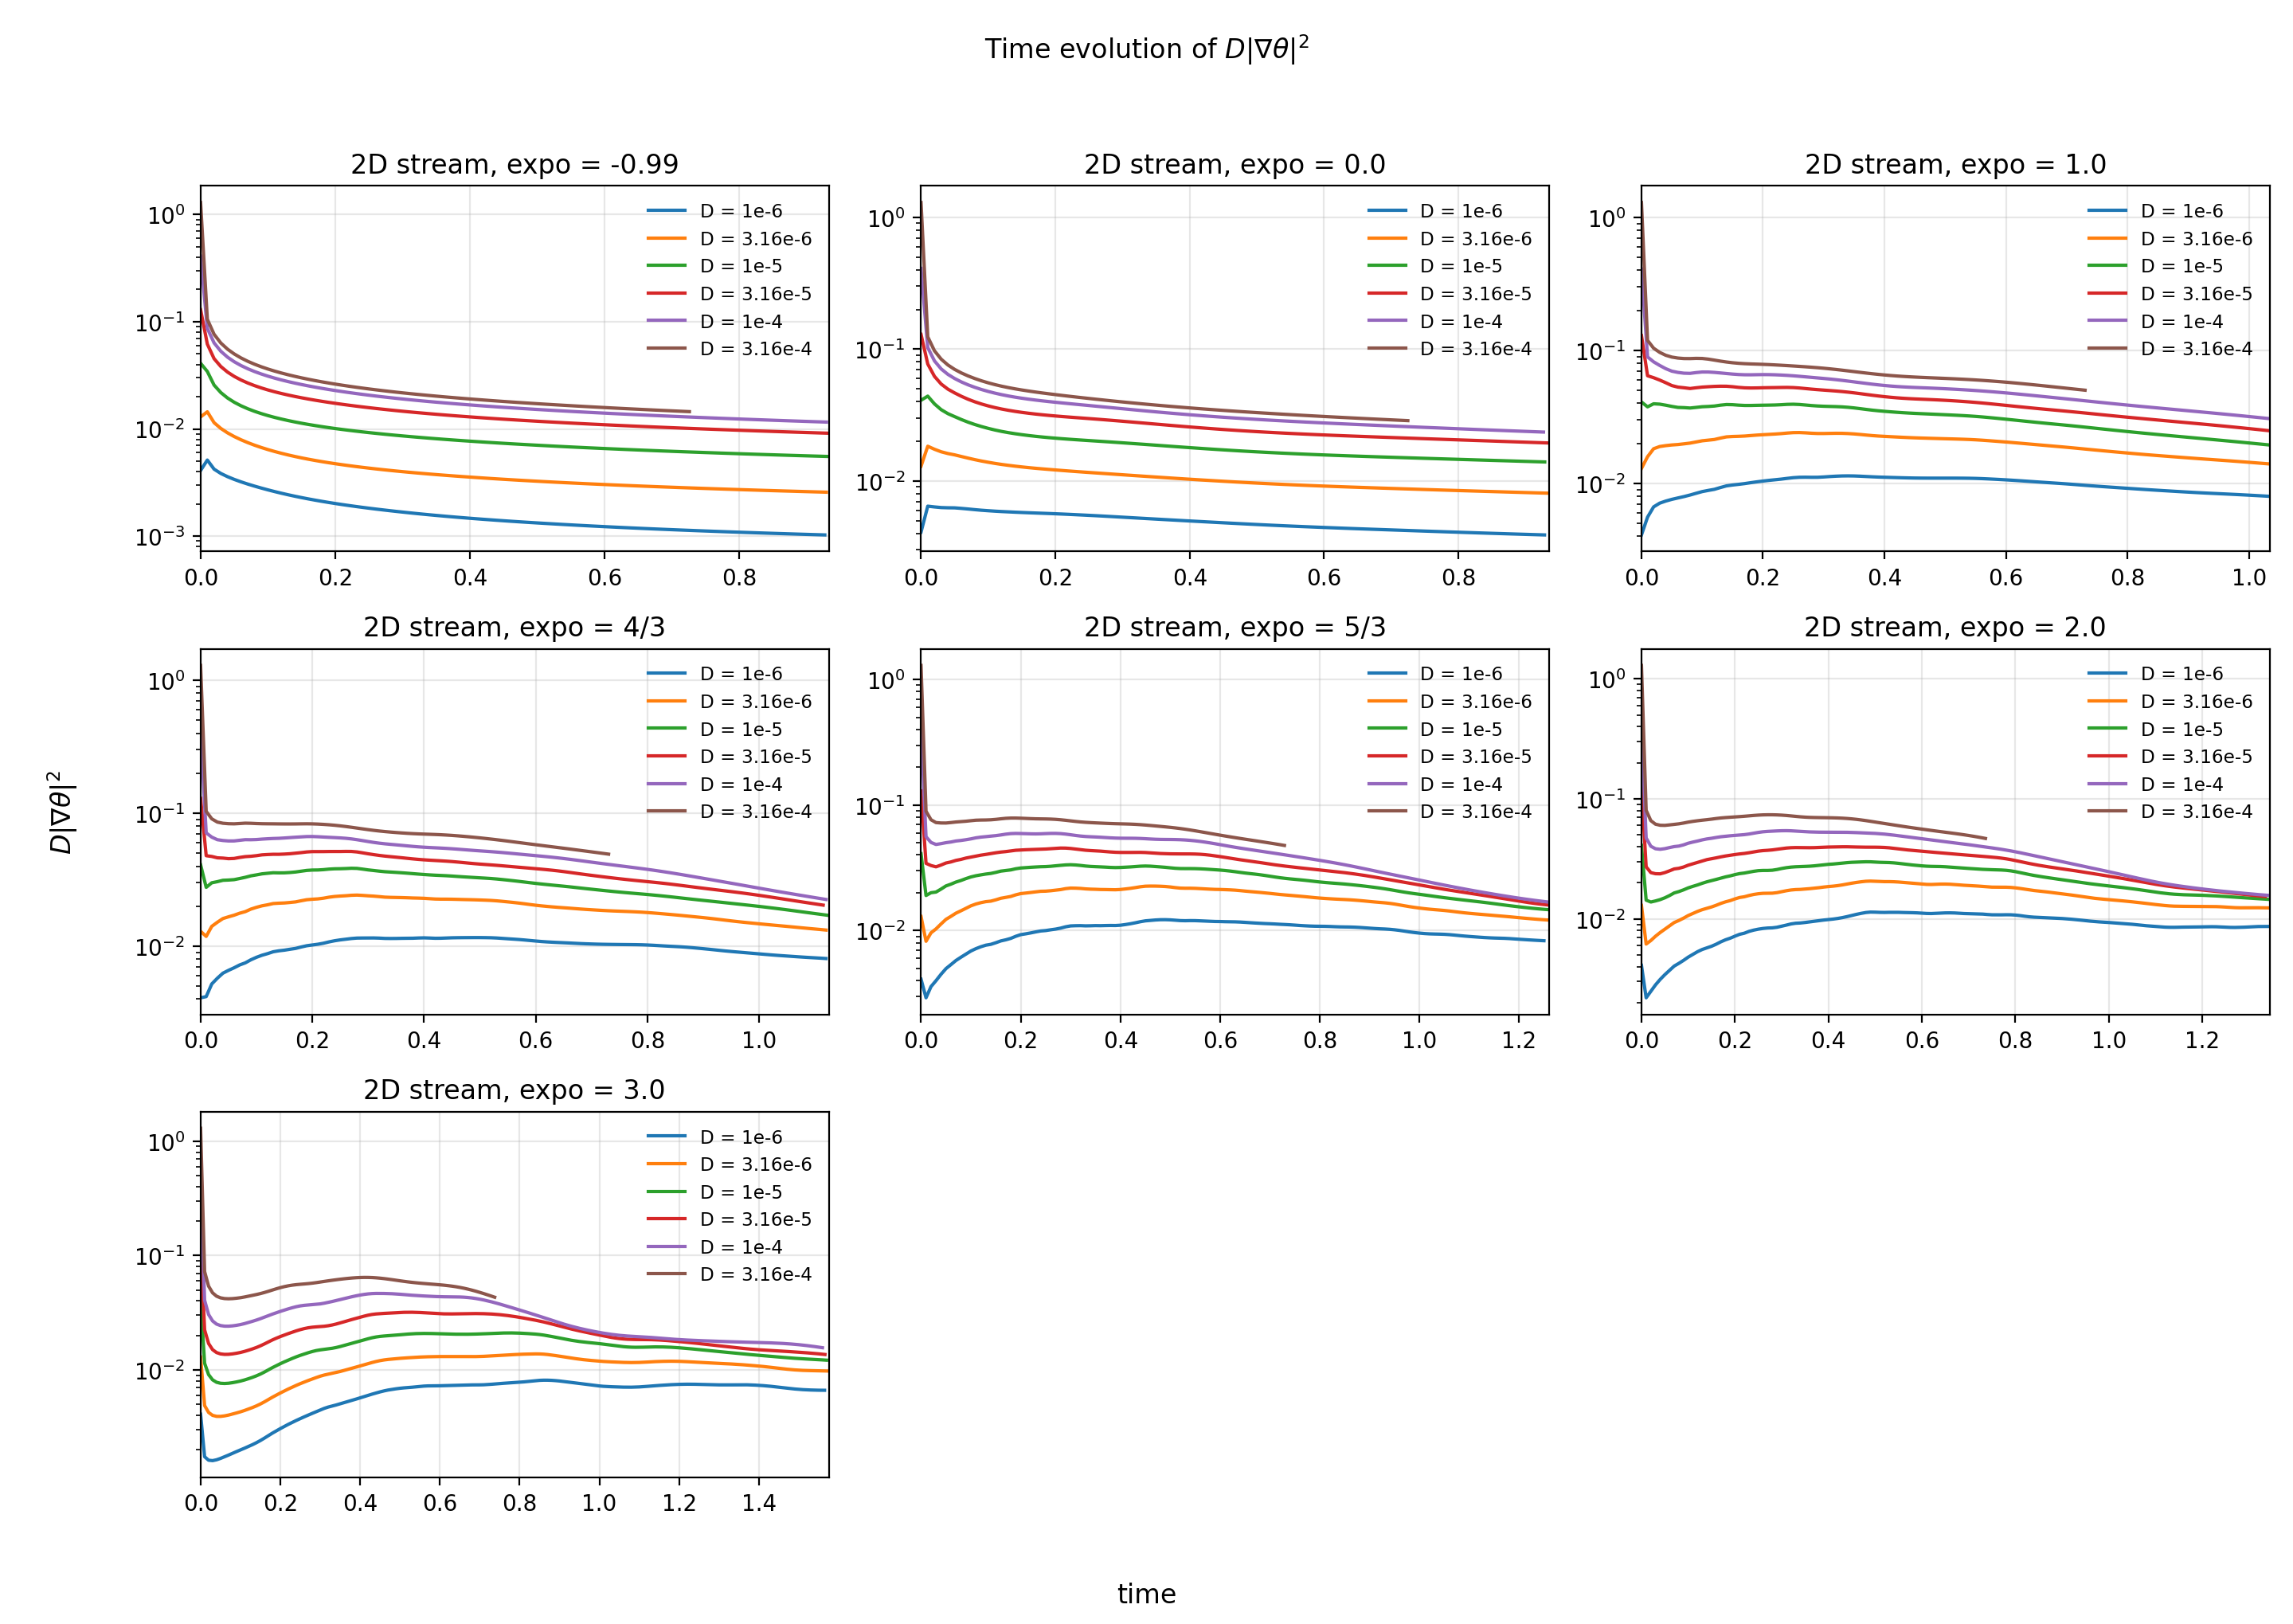
\includegraphics[width=0.80\textwidth]{figures_perfect1_step_rapidsine/chi_vs_time_s_00_2d.png}
    \caption{2D stream-function runs.}
  \end{subfigure}

  \vspace{0.75em}

  \begin{subfigure}[t]{\textwidth}
    \centering
    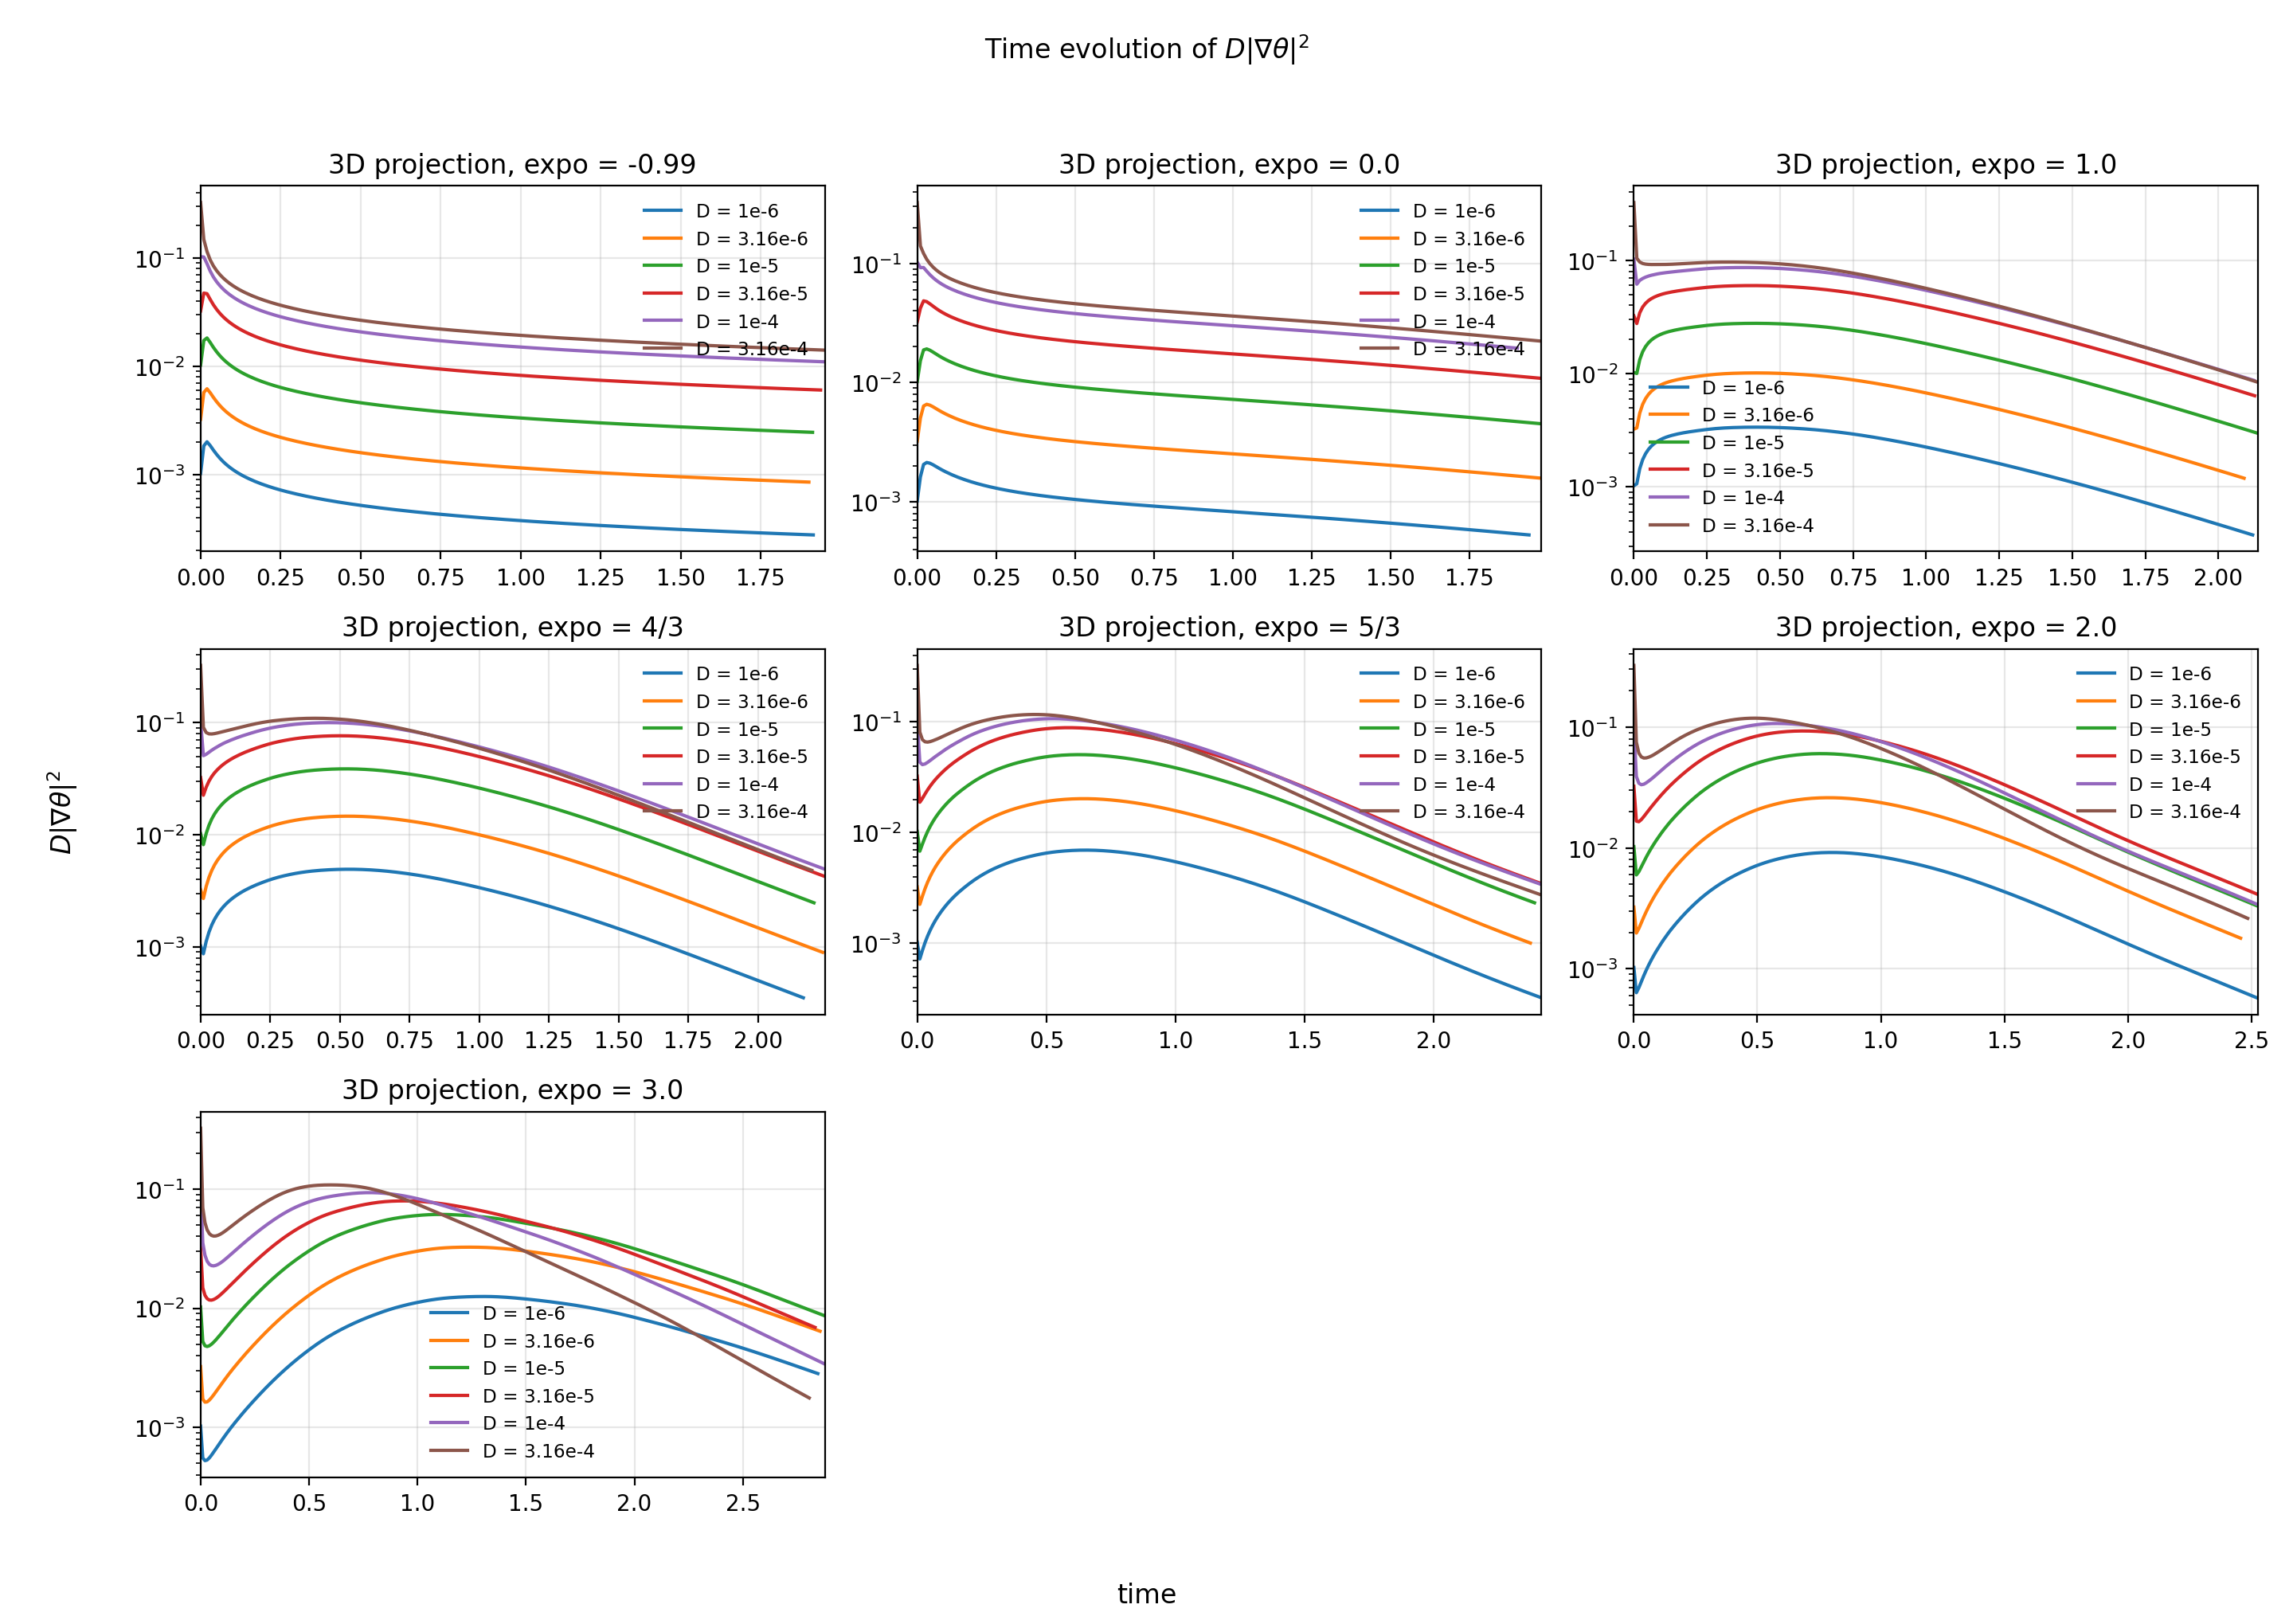
\includegraphics[width=0.80\textwidth]{figures_perfect1_step_rapidsine/chi_vs_time_s_00_3d.png}
    \caption{3D projection runs.}
  \end{subfigure}
  \caption{Instantaneous scalar-dissipation diagnostics as a function of time. These
  traces show when dissipation is active during the run and how the timing and
  amplitude shift with the velocity roughness.}
  \label{fig:chi-time}
\end{figure}

\begin{figure}[p]
  \centering
  \begin{subfigure}[t]{\textwidth}
    \centering
    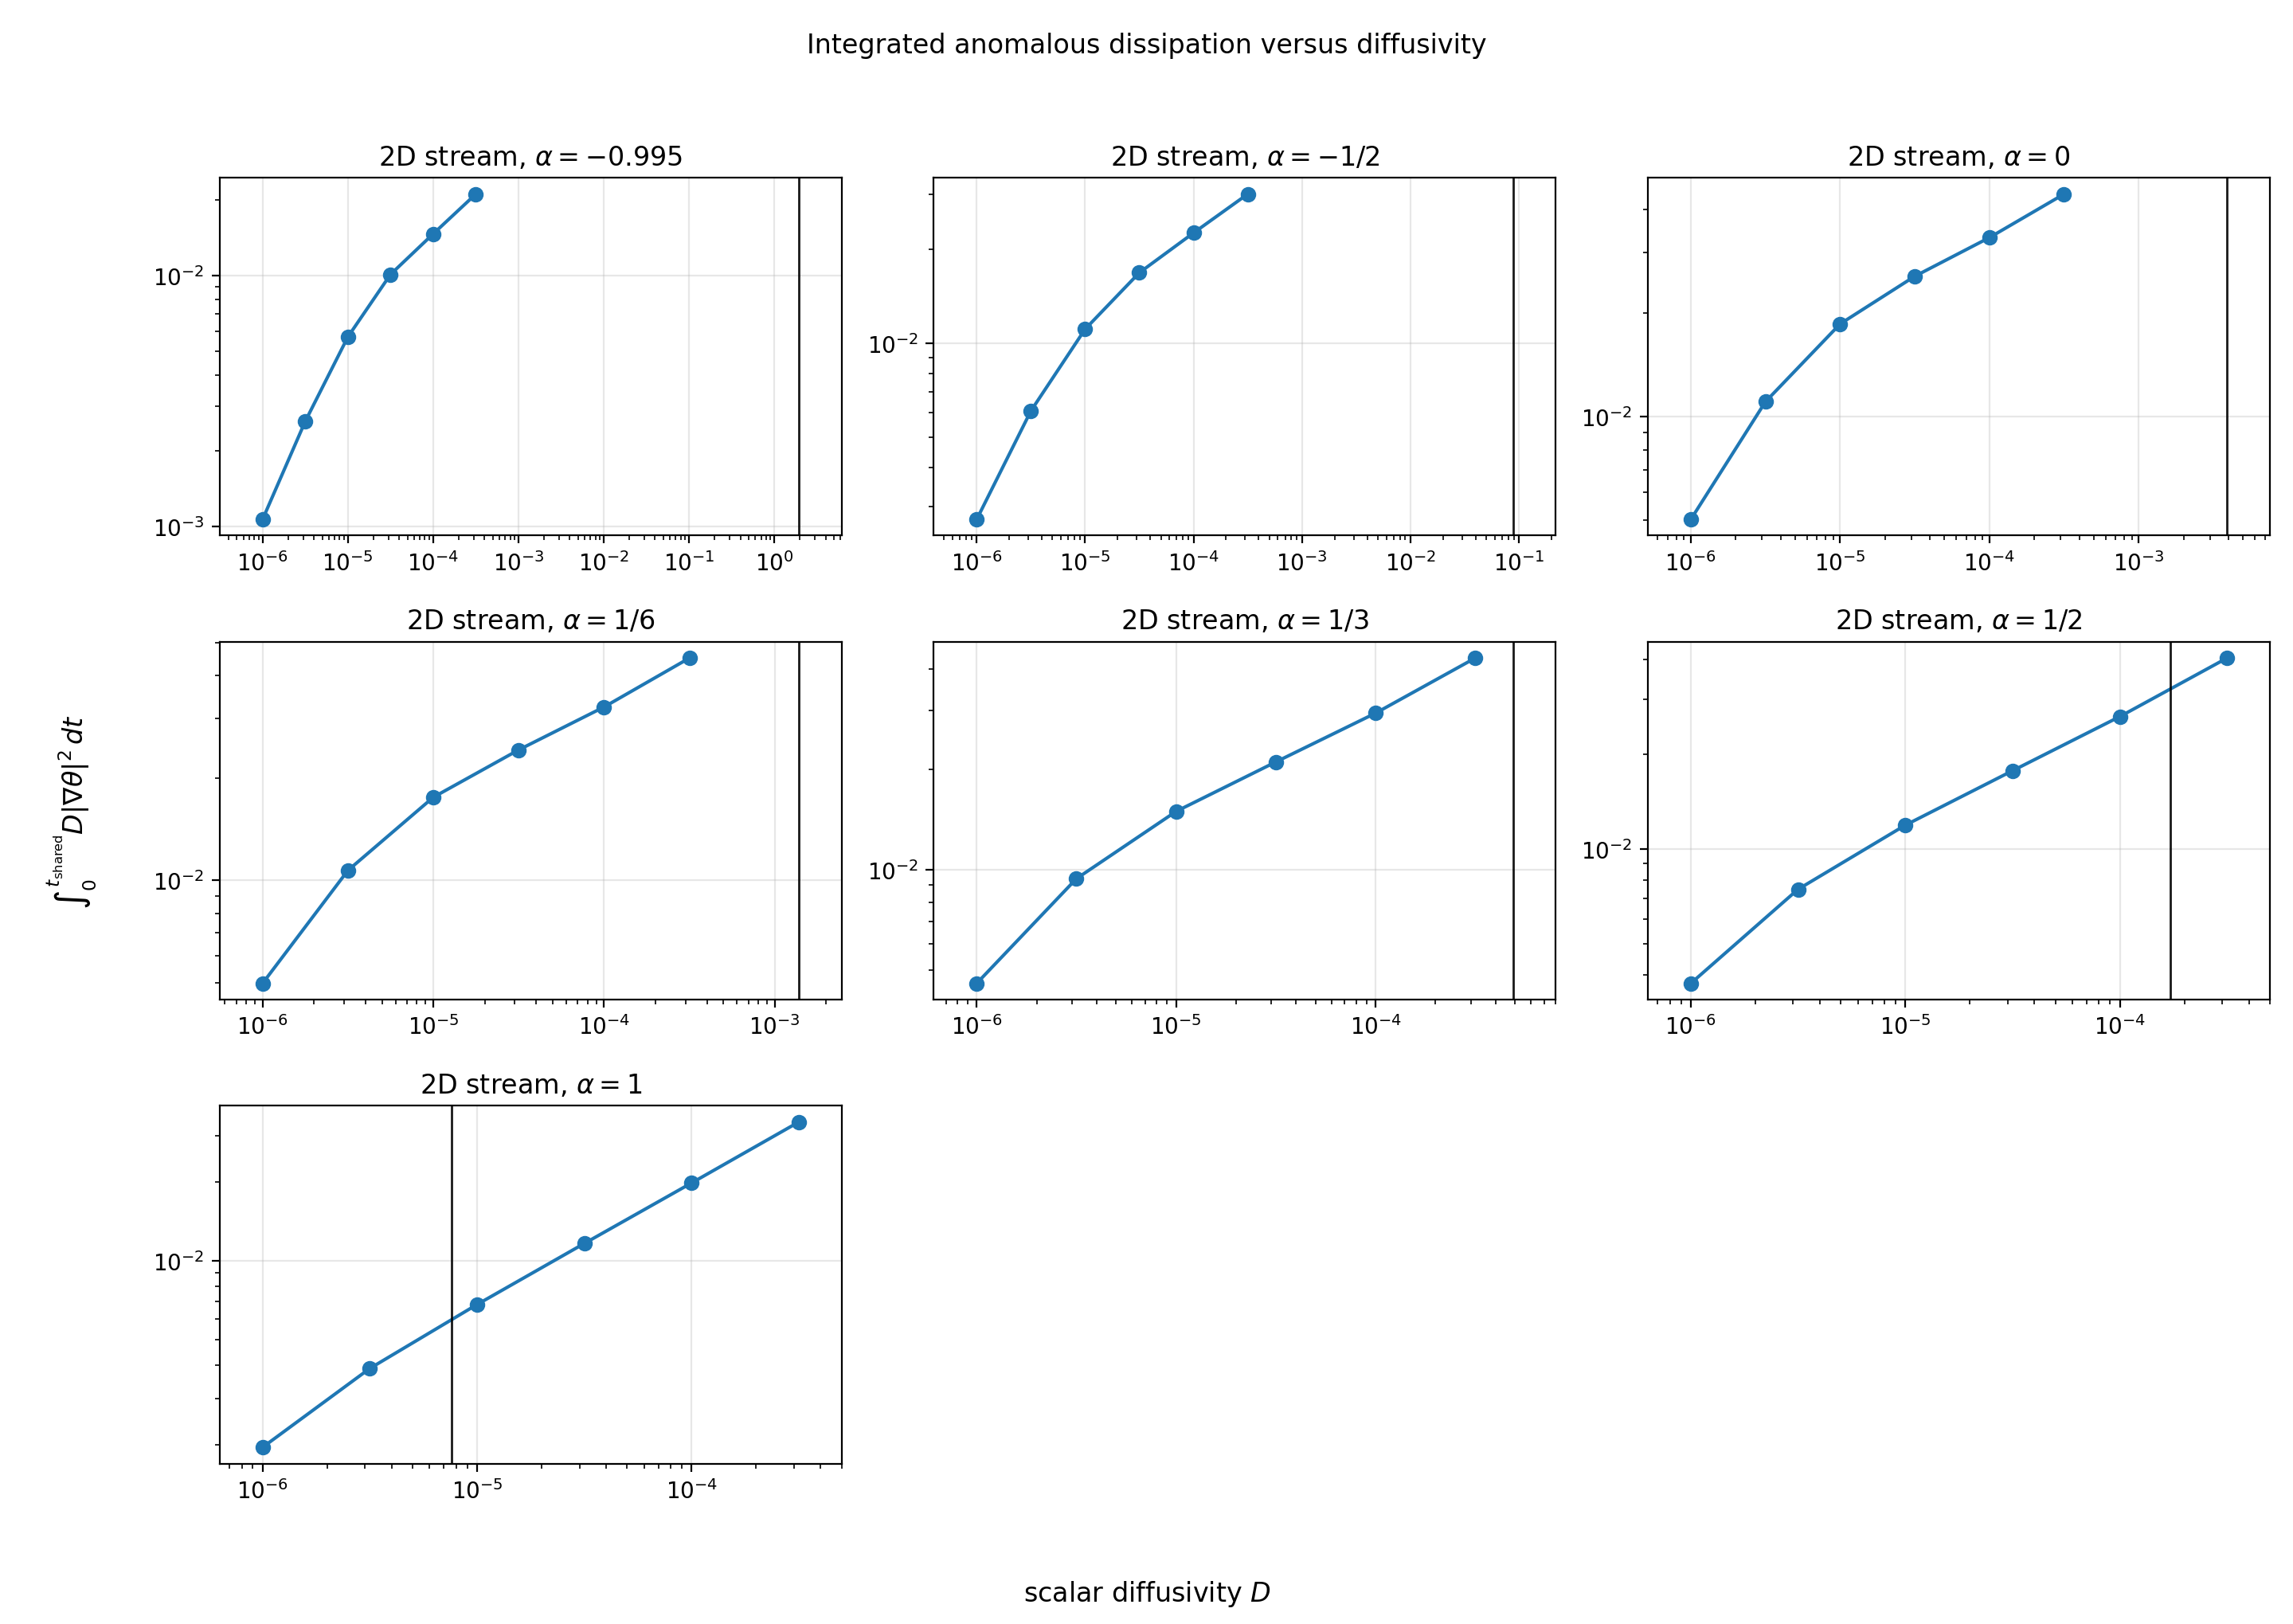
\includegraphics[width=0.80\textwidth]{figures_perfect1_step_rapidsine/anomalous_dissipation_integrated_vs_diffusivity_s_00_2d_shared.png}
    \caption{2D stream-function runs.}
  \end{subfigure}

  \vspace{0.75em}

  \begin{subfigure}[t]{\textwidth}
    \centering
    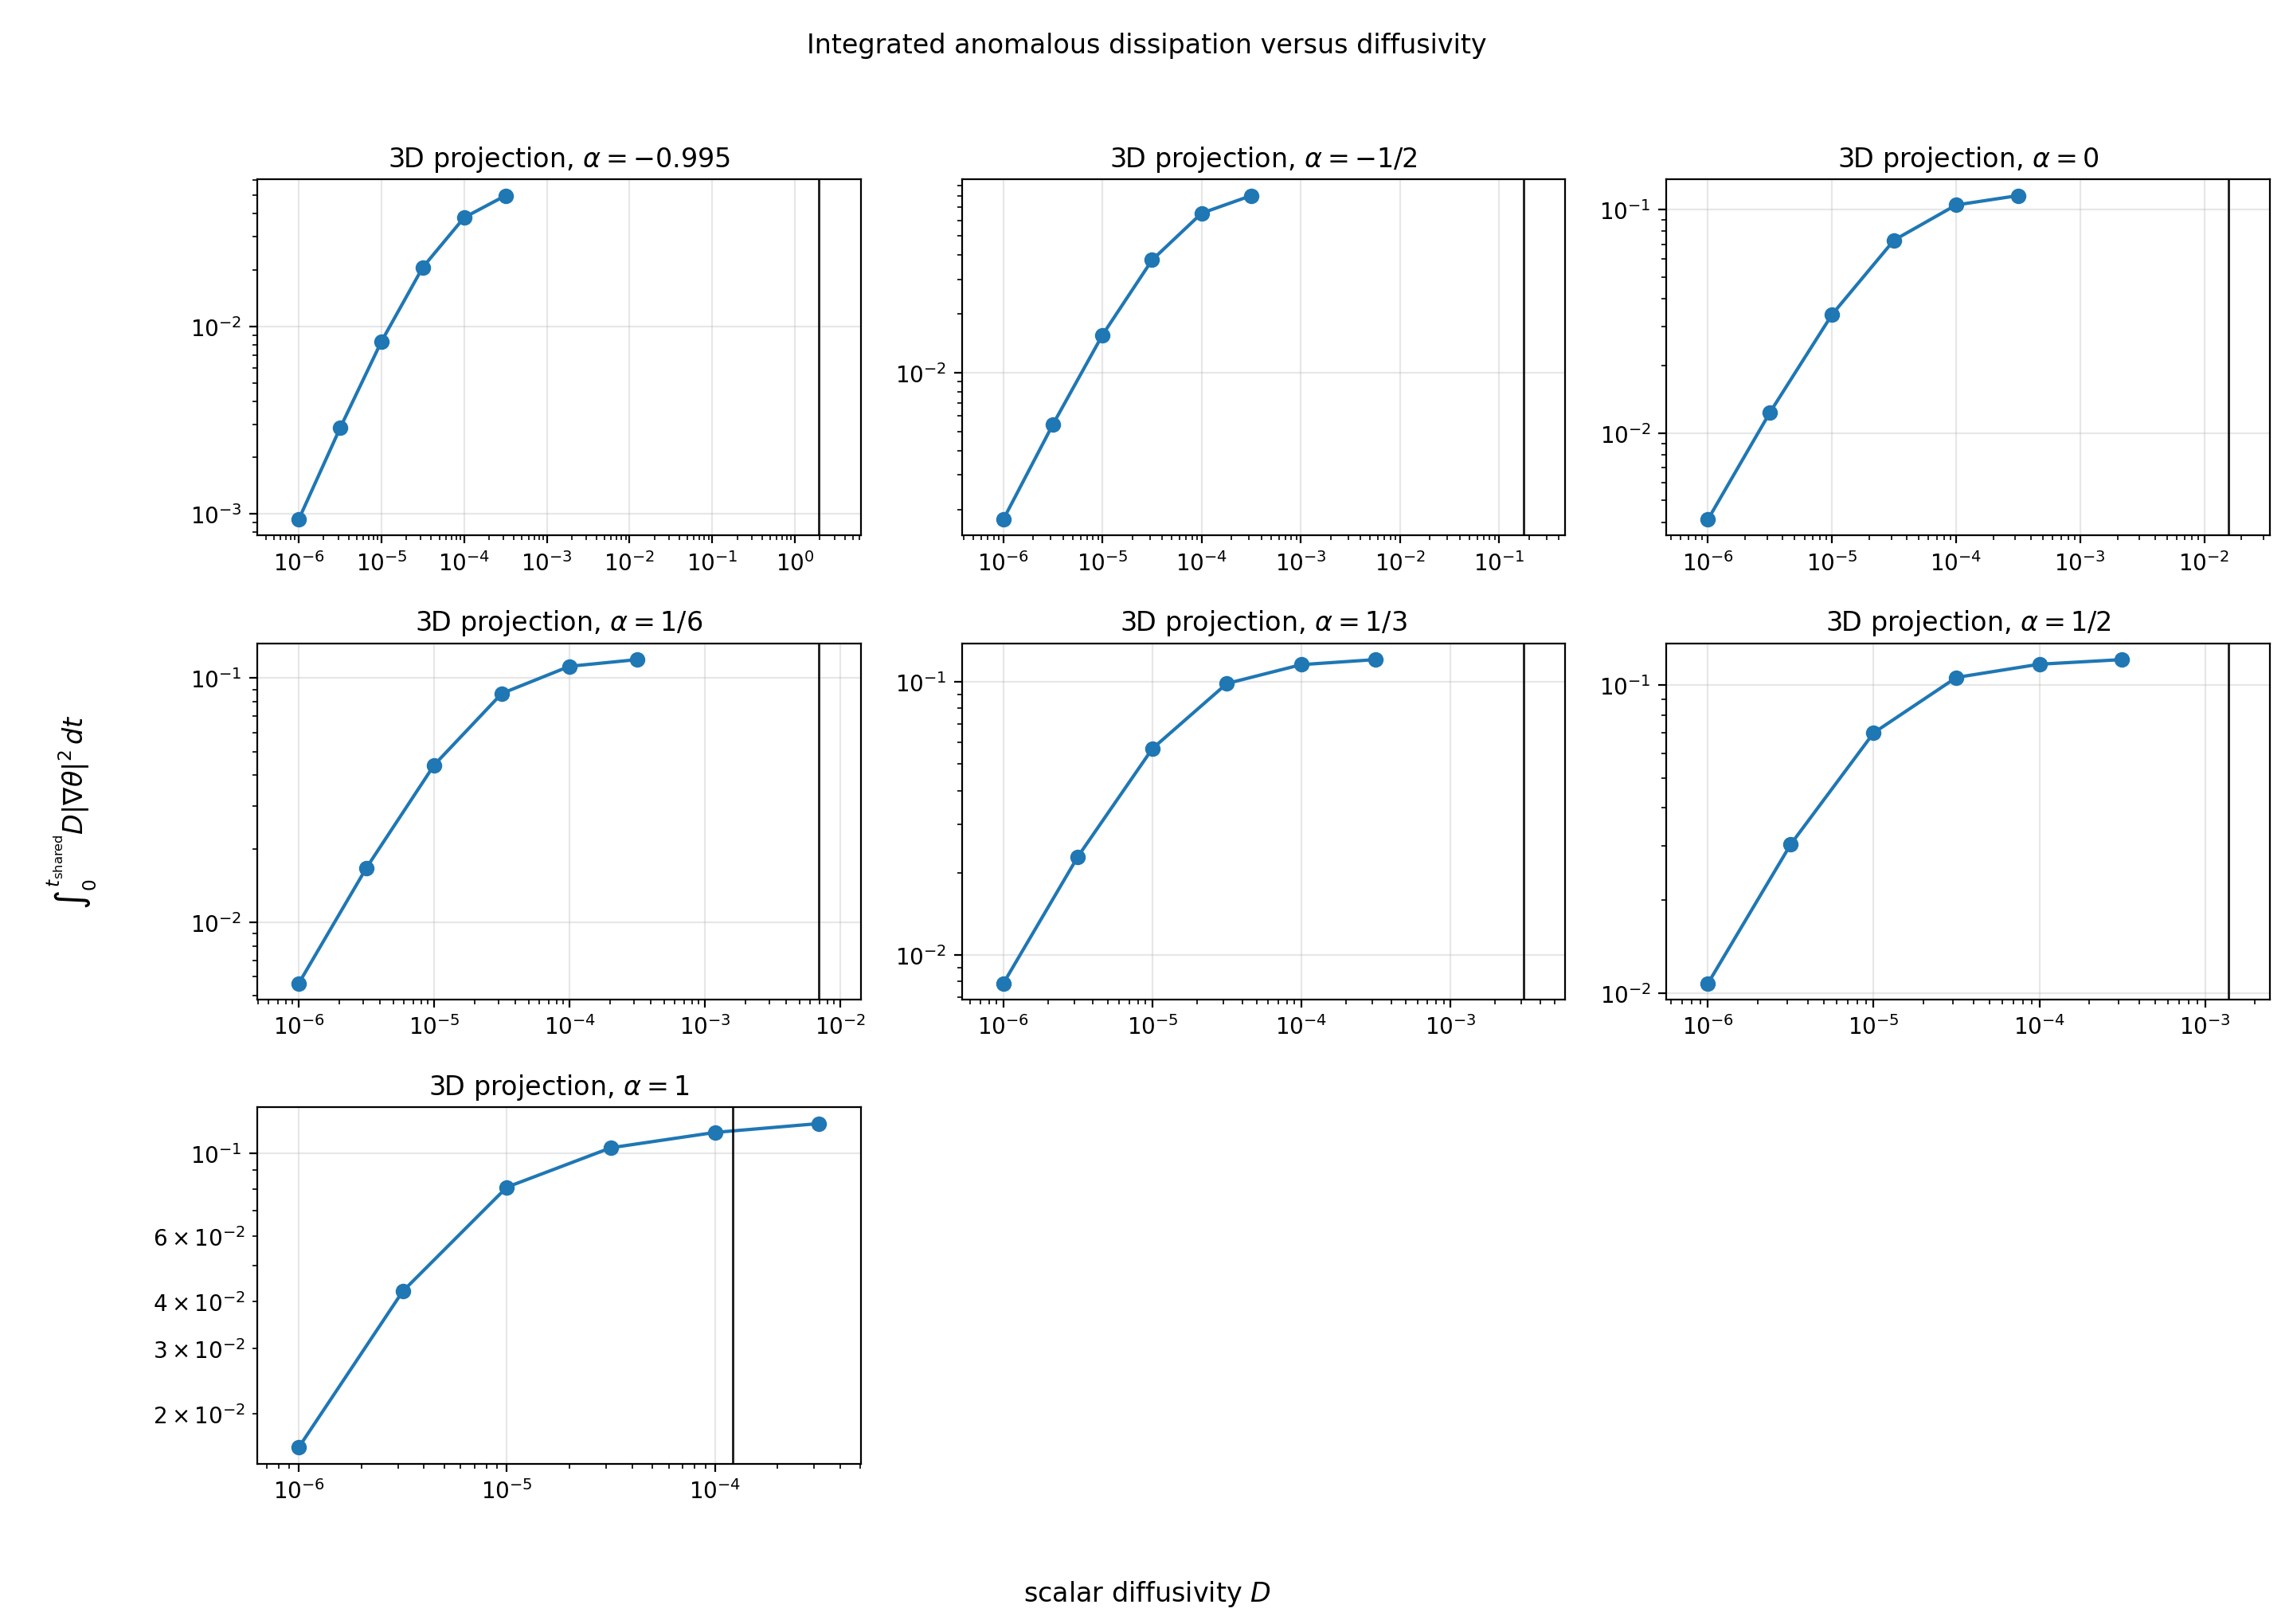
\includegraphics[width=0.80\textwidth]{figures_perfect1_step_rapidsine/anomalous_dissipation_integrated_vs_diffusivity_s_00_3d_shared.png}
    \caption{3D projection runs.}
  \end{subfigure}
  \caption{Finite-time integrated scalar dissipation as a function of diffusivity.
  The black vertical lines mark the estimated $D_{\min}$ threshold discussed in
  Figure \ref{fig:diff-range}; points to the left of those lines sit below the
  nominally admissible lower limit and should therefore be interpreted with caution.}
  \label{fig:chi-int}
\end{figure}

\FloatBarrier
\section{Takeaway}
Taken together, these figures document how scalar roughness and finite-time
dissipation vary with the imposed velocity roughness $\alpha$ and scalar diffusivity
$D$ in the 2D stream-function and 3D projection ensembles. The qualitative trends in
the spectra, the $\beta(\alpha)$ summaries, and the dissipation plots are all useful,
but the new diffusivity-range figure changes how the scan should be read: a large
fraction of the original diffusivity values lie outside the preferred buffered
window. The safest interpretation is therefore comparative rather than absolute. The
figures identify how the two ensembles respond across the scan, while the admissible
range estimate marks which parts of that scan should carry the most weight in later
physical conclusions.

A follow-up sweep is now being run with diffusivities targeted inside the buffered
optimal window identified in Figure \ref{fig:diff-range}. That next campaign also
replaces the discontinuous Heaviside initial condition with smooth sinusoidal initial
data, so the next comparison will probe the same roughness trends in a regime that
is both better aligned with the diffusivity constraints and less sensitive to the
sharp initial scalar jump.

\end{document}
